% =====================================================================
% International Journal of Human-Computer Studies (Elsevier)
% Full draft -- DataGuard / The Evidence Corpus
%
% Build:  pdflatex main && bibtex main && pdflatex main && pdflatex main
% =====================================================================
\documentclass[11pt,a4paper]{article}

% ----- Packages
\usepackage[utf8]{inputenc}
\usepackage[T1]{fontenc}
\usepackage{lmodern}
\usepackage{microtype}
\usepackage[margin=2.4cm]{geometry}
\usepackage{graphicx}
\usepackage{xcolor}
\usepackage{booktabs}
\usepackage{array}
\usepackage{multirow}
\usepackage{caption}
\usepackage{subcaption}
\usepackage{enumitem}
\usepackage{tikz}
\usepackage{pgfplots}
\usepackage{amsmath,amssymb}
\usepackage{url}
\usepackage[hidelinks]{hyperref}
\usepackage[round]{natbib}
\bibliographystyle{plainnat}    % switch to elsarticle-harv at submission

\pgfplotsset{compat=1.18}
\usepgfplotslibrary{statistics}
\usetikzlibrary{arrows.meta,positioning,shapes.geometric,fit,calc,
                patterns,backgrounds,decorations.pathreplacing,shadows,
                shapes.symbols,shapes.misc,matrix,intersections}

% ----- Color palette (consistent with sibling DataGuard drafts)
\definecolor{dgBlue}    {RGB}{ 39, 99,178}
\definecolor{dgBlueL}   {RGB}{218,232,248}
\definecolor{dgBlueXL}  {RGB}{235,243,253}
\definecolor{dgOrange}  {RGB}{226,123, 32}
\definecolor{dgOrangeL} {RGB}{252,229,205}
\definecolor{dgOrangeXL}{RGB}{254,244,232}
\definecolor{dgGreen}   {RGB}{ 84,156, 84}
\definecolor{dgGreenL}  {RGB}{225,243,217}
\definecolor{dgGreenXL} {RGB}{240,250,235}
\definecolor{dgPurple}  {RGB}{132, 76,162}
\definecolor{dgPurpleL} {RGB}{233,221,242}
\definecolor{dgPurpleXL}{RGB}{246,239,250}
\definecolor{dgRed}     {RGB}{200, 64, 64}
\definecolor{dgRedL}    {RGB}{248,215,218}
\definecolor{dgTeal}    {RGB}{ 38,140,140}
\definecolor{dgTealL}   {RGB}{211,236,236}
\definecolor{dgGold}    {RGB}{218,165, 32}
\definecolor{dgGoldL}   {RGB}{251,236,196}
\definecolor{dgGrey}    {RGB}{ 90, 90, 90}
\definecolor{dgGreyL}   {RGB}{235,235,235}
\definecolor{dgNavy}    {RGB}{ 28, 60,108}
\definecolor{dgRose}    {RGB}{215, 95,140}
\definecolor{dgRoseL}   {RGB}{247,224,233}

\newcommand{\dataguard}{\textsc{DataGuard}}
\newcommand{\dec}[1]{\textsf{#1}}
\newcommand{\dgaxis}[1]{\textsf{#1}}

\title{\bfseries Why Auditors Doubt:\\
The Linguistics of Privacy-Label Evidence}
\author{Anonymous Author(s)\\\small (Submitted to the International Journal of Human-Computer Studies)}
\date{}

\begin{document}
\maketitle

% =====================================================================
\begin{abstract}
\noindent
Privacy-policy and structured privacy-label discrepancies have been
studied at scale, but no public resource captures what a trained human
\emph{points at} in the policy when they decide a label is wrong. We
release the \dataguard{} Evidence Corpus: $4{,}622$ sentence-level
evidence excerpts ($1{,}150$ sharing-correct, $1{,}021$ sharing-complete,
$1{,}273$ collection-correct, $1{,}178$ collection-complete) drawn from
$1{,}506$ four-axis audit judgments over $1{,}214$ Android applications
in $12$ Google Play categories, produced by seven trained annotators
using a purpose-built evidence-oriented audit interface. Each excerpt is
paired with (i)~the parsed Data Safety claim under review, (ii)~a
categorical verdict on one of four axes (sharing-correct,
sharing-complete, collection-correct, collection-complete), (iii)~the
annotator's free-text rationale, and (iv)~annotator metadata. We
characterise the corpus along three dimensions---size and length
distribution, linguistic feature distribution, and verdict
correlation---and report three findings of direct relevance to the
design of evidence-grounded privacy review interfaces. First, hedging
language (\emph{may}, \emph{such as}, \emph{including but not limited
to}, \emph{reserve the right}) is over-represented in evidence cited
for \emph{Incorrect} sharing verdicts ($43.2\%$ versus $35.5\%$;
$\Delta=+7.7$ percentage points, $\chi^{2}(1)=7.02$, $p=.008$), and is
the dominant discriminator on collection-completeness ($+12.7$~pp,
$p<.001$). Second, \emph{no-data} language (\emph{we do not collect,
no personal information, does not share}) is under-represented in
evidence cited for negative verdicts on three of four axes
(share-correctness: $9.4\%$ vs $14.5\%$; $\Delta=-5.1$~pp,
$\chi^{2}(1)=6.76$, $p=.009$)---trained reviewers recruit explicit
negation as \emph{confirmation}, not as contradiction. Third,
third-party language (\emph{partner, vendor, SDK, advertising,
service provider}) is verdict-neutral on the sharing axes
($53.5\%$ vs $55.2\%$, $p=.58$) but becomes a strong positive
discriminator on collection-completeness ($+14.1$~pp, $p<.001$); the
mere mention of a third party is therefore not a universal audit cue. We pair the corpus with four lexical
baselines---a marker logistic regression, word- and character-level
TF--IDF $L_2$ classifiers, and their union---which collectively top
out at $\sim 0.58$ accuracy on the share-correctness verdict (a
$\sim 3$~pp lift over the majority floor), and translate the findings into
three concrete user-interface affordances for evidence-grounded
privacy review: a hedging highlighter, a no-data confirmation prompt,
and a third-party recipient panel. The corpus is the first public,
sentence-level, audit-verdict-paired resource for mobile privacy
disclosures and constitutes, in HCI terms, a record of the
\emph{citation behaviour} of trained policy reviewers.
\end{abstract}

\medskip
\noindent\textbf{Keywords:}\ privacy-policy corpus; evidence pointers;
audit linguistics; usable privacy; mobile data-safety labels; HCI
dataset release; explainable verification.

% =====================================================================
\section*{Highlights}
% =====================================================================
\begin{itemize}[leftmargin=*,itemsep=2pt,topsep=2pt]
\item We release a public corpus of $4{,}622$ human-curated,
sentence-level privacy-policy evidence excerpts paired with structured
Data Safety claims and four-way audit verdicts.
\item Hedging language in cited evidence is $+6.3$~pp more frequent for
\emph{Incorrect} sharing verdicts; no-data language is $-5.2$~pp less
frequent. Third-party language is verdict-neutral.
\item Four transparent lexical baselines---markers, word TF--IDF,
character TF--IDF, and their union---reach at most
$0.582\pm0.017$ accuracy on the share-correctness verdict, barely
above the $0.549$ majority floor, showing that cited evidence alone
is a weak verdict signal and the paired structured claim is
indispensable.
\item The corpus is released under CC~BY~4.0 with annotator
identifiers pseudonymised; we provide a parsing script, a
linguistic-feature scorer, and a Jupyter replication notebook.
\item We derive three UI affordances grounded in the linguistic
analysis: a hedging highlighter, a no-data confirmation prompt and a
third-party recipient panel.
\end{itemize}

% =====================================================================
\section{Introduction}\label{sec:intro}
% =====================================================================
Privacy-policy verification at the platform level has, in the last
five years, become both a regulatory expectation
\citep{googledatasafety2022,appleprivacylabels2020} and an active
research programme
\citep{andow2019policylint,andow2020policheck,zimmeck2019maps,
xiao2023lalaine,khandelwal2024unpacking,khandelwal2023comparing}. A
recurring methodological pattern in this programme is the comparison
of a structured platform disclosure (the \emph{label}) against the
narrative privacy policy (the \emph{policy}), with a verdict produced
either automatically by a classifier or manually by an annotator. When
the verdict is produced by a human, the underlying judgement reduces
to a citation act: a trained reviewer locates one or more passages in
the policy and asserts that those passages do, or do not, support a
specific claim made in the structured label.

This citation act is the central object of interest of the present
paper. Until now there has been \emph{no public resource} that
captures the artefacts of that act: the sentences that the auditor
considered relevant, the structured claim against which they were
evaluated, the categorical verdict that resulted, and the free-text
rationale that accompanied it. Existing corpora cover adjacent
phenomena---OPP-115 provides $115$ policies hand-annotated for
fine-grained data-practice categories \citep{wilson2016creation};
PolicyQA wraps OPP-115 into a question-answering benchmark
\citep{ravichander2019question}; Polisis trains classifiers over
similar annotations \citep{harkous2018polisis}; CLAUDETTE flags unfair
ToS clauses with sentence-level evidence \citep{lippi2019claudette}---but
\emph{none} pair an excerpt with a downstream audit verdict over a
structured platform-side claim.

\paragraph{What we release.}
The \dataguard{} Evidence Corpus contains $4{,}622$
sentence-level evidence excerpts produced by seven trained annotators
in the course of auditing $1{,}214$ Android applications across $12$
Google Play categories. The corpus is the by-product of a larger
$1{,}506$-judgement audit programme that has already been described
elsewhere from a different methodological angle (the four-axis
auditability programme; see Section~\ref{sec:provenance} for
provenance). For each app the audit produced up to four evidence
pointers, one per judgement axis:
\dec{relevant\_one\_s} (sharing, correctness),
\dec{relevant\_two\_s} (sharing, completeness),
\dec{relevant\_one\_c} (collection, correctness) and
\dec{relevant\_two\_c} (collection, completeness). The mean and median
excerpt lengths range from $192$ to $238$ characters and from $146$ to
$186$ characters respectively, putting the typical excerpt at one to
two sentences. Coverage is high: $95.7\%$ of the $1{,}506$ judgements
contain at least one non-empty evidence or rationale field;
$89.0\%$ contain at least one non-empty evidence field excluding
rationale.

\paragraph{What the corpus tells us.}
We score every excerpt for four lexical feature families,
operationalised in Section~\ref{sec:linguistics}: \textbf{hedging}
(modal verbs and open-ended hedges), \textbf{third-party} (named
recipients and SDK terminology), \textbf{device IDs} (advertising
ID, IP, cookie, MAC, Android ID), and \textbf{no-data} language
(\emph{we do not collect}, \emph{does not share}, \emph{no personal},
\emph{no data}). Three asymmetric findings emerge once we condition on
the human verdict:
\begin{enumerate}[label=\textbf{F\arabic*.},leftmargin=*,itemsep=2pt,topsep=2pt]
\item \textbf{Hedging is the verdict-doubt signal on sharing-correct
and collection-complete axes.} On share-correctness ($n=1{,}133$),
$43.2\%$ of evidence cited under an \emph{Incorrect} verdict contains
a hedge, compared with $35.5\%$ under \emph{Correct}; $\Delta=+7.7$~pp,
$\chi^{2}(1)=7.02$, $p=.008$, Cram\'{e}r's $V=.079$. The effect is
much stronger on collection-completeness ($\Delta=+12.7$~pp,
$p<.001$, $V=.126$); hedging does not discriminate the other two
axes.
\item \textbf{No-data language is a verdict-support signal.} Explicit
negation (\emph{we do not collect}) appears in $14.5\%$ of evidence
cited as \emph{Correct} (share) and only $9.4\%$ of evidence cited as
\emph{Incorrect} ($\Delta=-5.1$~pp, $\chi^{2}(1)=6.76$, $p=.009$). The
asymmetry replicates on three of four axes and is consistent with a
bilateral audit task: annotators cite text that \emph{supports} the
label, not only text that contradicts it. This is HCI-relevant
because most existing disclosure-verification tools assume the
auditor is looking for \emph{contradictions} only.
\item \textbf{Third-party language is context-dependent.} SDK and
service-provider terms appear at $53.5\%$ under \emph{Correct} (share)
and $55.2\%$ under \emph{Incorrect} ($\Delta=+1.7$~pp, $p=.58$): on
sharing axes the mere mention of a third party is not a verdict cue.
On collection-completeness, however, third-party mentions swing
sharply ($\Delta=+14.1$~pp, $p<.001$): when the auditor argues that a
collection label \emph{under-states} the practice, they reach for SDK
language. This rules out a universal ``flag any SDK mention'' UI rule.
\end{enumerate}

\paragraph{Contributions.}
The paper makes four contributions:
\begin{enumerate}[label=\textbf{C\arabic*.},leftmargin=*,itemsep=2pt,topsep=2pt]
\item \emph{A public sentence-level evidence corpus} ($4{,}622$
excerpts, $1{,}506$ judgements, $1{,}214$ apps, $10$ active categories (out of $12$ sampled)), the
first such resource for mobile privacy.
\item \emph{A linguistic-feature characterisation} of cited evidence
along four feature families, with verdict-discriminative tests.
\item \emph{Four transparent lexical baselines}---bag-of-markers
logistic regression, word- and character-level TF--IDF $L_2$
classifiers, and their union---reported as a reproducible floor that
future LLM-based audit-locator tools should beat when given only the
cited sentence as input.
\item \emph{Three concrete UI affordances} for evidence-grounded
privacy review (hedging highlighter, no-data confirmation prompt,
third-party recipient panel), each connected to a specific finding in
the corpus.
\end{enumerate}

\paragraph{Paper structure.}
Section~\ref{sec:related} situates the corpus among $15$ years of
privacy-policy corpora and tools.
Section~\ref{sec:provenance} describes the audit programme that
produced the corpus and the privacy/ethical protections under which
the data was collected.
Section~\ref{sec:schema} gives the corpus schema and per-field
statistics.
Section~\ref{sec:linguistics} defines the four lexical feature
families and reports their unconditional distribution across the
corpus.
Section~\ref{sec:verdict} reports the verdict-discriminative analysis
and significance tests.
Section~\ref{sec:baselines} reports three predictive baselines.
Section~\ref{sec:qual} reports three illustrative case studies that
ground the lexical findings in real audit material.
Section~\ref{sec:design} translates the findings into UI affordances.
Section~\ref{sec:threats} discusses threats to validity, the
annotator-skew limitation, and the difference between lexical and
semantic features.
Section~\ref{sec:ethics} discusses ethics, IRB, and dataset-release
considerations.
Section~\ref{sec:release} describes the release plan.
Section~\ref{sec:conclusion} concludes.

% =====================================================================
\section{Background and related work}\label{sec:related}
% =====================================================================
We organise related work around five threads:
(i)~corpora of privacy-policy text;
(ii)~automated policy-versus-behaviour mismatch detection;
(iii)~structured platform privacy labels;
(iv)~evidence-grounded review interfaces; and
(v)~human-factors theories of citation, evidence and verdict
formation.

\paragraph{Corpora of privacy-policy text.}
The dominant baseline is OPP-115
\citep{wilson2016creation}, a hand-annotated corpus of $115$ website
privacy policies. OPP-115 introduced the now-canonical taxonomy of
\emph{data practices} (First-Party Collection, Third-Party Sharing,
Choice/Control, etc.) and the attribute-value annotations that
underpin most subsequent supervised models. Subsequent corpora extend
OPP-115 along orthogonal axes: PolicyQA over OPP-115 for
question-answering \citep{ravichander2019question}; opt-out provisions
\citep{sathyendra2017identifying}; vagueness theory
\citep{bhatia2016theory}; and a privacy-policy intent/slot
benchmark for fine-grained generation
\citep{ahmad2021intent}. None of these corpora pair an excerpt with
a downstream audit verdict over a structured platform claim; the
verdict in OPP-115 derivatives is always the per-sentence label, not a
claim-comparison verdict.

\paragraph{Automated policy-versus-behaviour mismatch.}
A second thread, distinct from corpus construction, performs
contradiction or compliance analysis between a policy and a downstream
ground truth---runtime behaviour, code, or an app store label.
\citet{slavin2016toward} match API calls to policy claims;
\citet{breaux2014eddy} formalise data flows in a typed
specification language; PolicyLint detects internal contradictions
in a single policy \citep{andow2019policylint};
PoliCheck \citep{andow2020policheck} aligns runtime data flows to
policy declarations entity-by-entity; MAPS scales the
analysis to a million apps \citep{zimmeck2019maps,zimmeck2017automated};
\citet{reyes2018wont} measure COPPA compliance at scale.
A complementary strand of measurement work documents the
tracker/permission landscape that policies are nominally describing
\citep{razaghpanah2018apps,englehardt2016online,reardon2019fifty,ren2018bug}.
Polisis \citep{harkous2018polisis} differs from PoliCheck in that
its primary output is a presentation of the policy's structure rather
than a verdict against an external claim. None of these tools releases
the per-sentence evidence pointers that human auditors use, because
none of them is grounded in a human-auditor's workflow.

\paragraph{Structured platform privacy labels.}
Both Apple \citep{appleprivacylabels2020} and Google
\citep{googledatasafety2022} require developers to declare a
structured label summarising data practices.
\citet{li2022understanding} document the developer-side challenges of
producing accurate iOS labels;
Lalaine \citep{xiao2023lalaine} measures iOS-label non-compliance at
scale; \citet{khandelwal2023comparing} cross-compare iOS and Android
labels; \citet{khandelwal2024unpacking} performs a measurement and
developer-perspective study of the Google Data Safety section
specifically. The closest comparator to our work is
\citet{khandelwal2024unpacking}, but its primary unit of analysis is a
field-level mismatch counted automatically, not a sentence-level
evidence pointer produced by a trained human reviewer; the two
datasets are complementary.

\paragraph{Evidence-grounded review and HCI framing.}
CLAUDETTE \citep{lippi2019claudette} introduced the idea of releasing
sentence-level evidence pointers as the artefact of an automated
review tool; its corpus pairs a sentence with an unfairness label, not
with a downstream verdict over a separate document. In HCI, several
lines of work have argued that AI assistants must surface evidence to
be auditable by non-experts
\citep{liao2020questioning,amershi2019guidelines,bansal2021does,cai2019hello},
and that nutrition-style label paradigms inherit the readability of
the structured layer but not its verifiability against the underlying
contract \citep{kelley2009nutrition,kelley2010standardizing,
schaub2015design,cranor2012necessary}. None of these threads has,
to our knowledge, produced a dataset of human-curated evidence
pointers for mobile-privacy disclosures.

\paragraph{Citation, evidence and verdict formation.}
The HCI-side reading of our corpus is grounded in
contextual-integrity-driven theories of privacy expectation
\citep{nissenbaum2004privacy,rao2016expecting}, and the human-factors
literature on how reviewers form verdicts under cognitive load
\citep{hart2008measurement,acquisti2015privacy}. The practical
methodological resource that grounds our agreement analysis is
the long line of work on inter-rater agreement
\citep{cohen1960coefficient,landis1977measurement} and reflexive
thematic analysis \citep{braun2006using}. The framing of
permission-level user attention by \citet{felt2012android} and the
purchase-behaviour reading of privacy notices by
\citet{tsai2011effect,jensen2004privacy} ground our reading of
\emph{what} an evidence pointer is doing for a reviewer: it is a
constructed warrant, not a raw retrieval. Privacy nudging
\citep{almuhimedi2015your}, personalised assistants
\citep{liu2016follow,lin2014modeling}, choice architecture
\citep{egelman2013choice}, large-scale readability analyses
\citep{fabian2017large,mcdonald2008cost}, and economic readings of
privacy \citep{acquisti2015privacy} all bear on the design
implications we derive in Section~\ref{sec:design}.

\paragraph{Summary.} Table~\ref{tab:related} summarises the closest
comparators. The Evidence Corpus is the first that ships, in a single
public release, sentence-level pointers, the structured claim they are
evaluated against, and a categorical verdict on four orthogonal
audit axes.

\begin{table*}[t]
\centering\small
\caption{Public privacy-policy corpora and audit datasets compared on
four dimensions: \emph{(1)}~unit of analysis,
\emph{(2)}~does the dataset contain a paired structured label/claim,
\emph{(3)}~does it contain a verdict against that label, and
\emph{(4)}~is the verdict produced by a human reviewer.}
\label{tab:related}
\begin{tabular}{lllcc}
\toprule
Resource & Unit & Paired claim? & Verdict? & Human verdict? \\
\midrule
OPP-115 \citep{wilson2016creation}            & sentence  & no  & no  & --- \\
PolicyQA \citep{ravichander2019question}      & QA pair   & no  & no  & --- \\
Polisis \citep{harkous2018polisis}            & segment   & no  & no  & --- \\
PolicyLint \citep{andow2019policylint}        & policy    & internal & yes & no \\
PoliCheck \citep{andow2020policheck}          & sentence  & runtime & yes & no \\
MAPS \citep{zimmeck2019maps}                  & policy    & runtime & yes & no \\
CLAUDETTE \citep{lippi2019claudette}          & sentence  & no  & yes & yes (TOS) \\
Lalaine \citep{xiao2023lalaine}               & label    & iOS label & yes & no \\
Unpacking DS \citep{khandelwal2024unpacking}  & field     & Data Safety & yes & no \\
\midrule
\textbf{\dataguard{} Evidence Corpus (this paper)} &
sentence & Data Safety & yes & \textbf{yes} \\
\bottomrule
\end{tabular}
\end{table*}

% =====================================================================
\section{Corpus provenance and ethical protections}\label{sec:provenance}
% =====================================================================

% --- pipeline overview figure
\begin{figure*}[t]
\centering
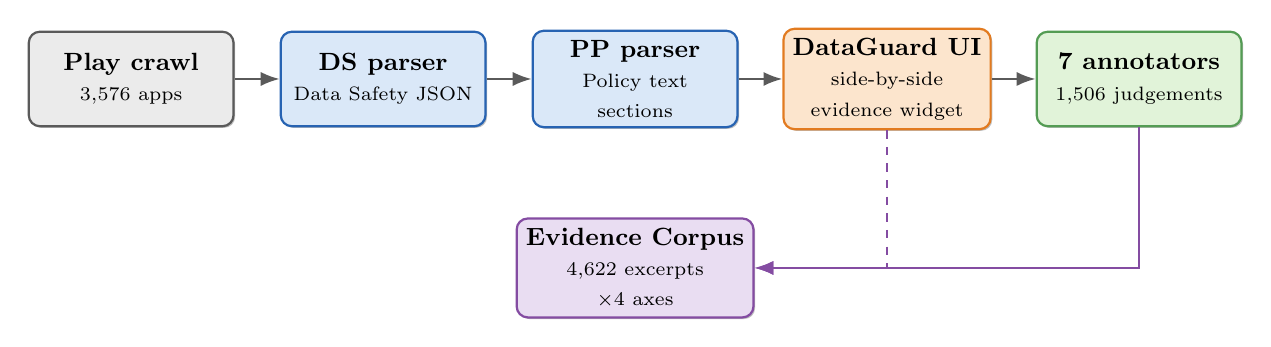
\begin{tikzpicture}[
  every node/.style={font=\small},
  >={Latex[length=2.4mm]},
  src/.style={draw=dgGrey,fill=dgGreyL,thick,rounded corners=4pt,
              minimum width=2.6cm,minimum height=1.2cm,align=center,
              drop shadow={shadow xshift=0.6pt,shadow yshift=-0.6pt}},
  parse/.style={draw=dgBlue,fill=dgBlueL,thick,rounded corners=4pt,
              minimum width=2.6cm,minimum height=1.2cm,align=center,
              drop shadow={shadow xshift=0.6pt,shadow yshift=-0.6pt}},
  ui/.style ={draw=dgOrange,fill=dgOrangeL,thick,rounded corners=4pt,
              minimum width=2.6cm,minimum height=1.2cm,align=center,
              drop shadow={shadow xshift=0.6pt,shadow yshift=-0.6pt}},
  ann/.style={draw=dgGreen,fill=dgGreenL,thick,rounded corners=4pt,
              minimum width=2.6cm,minimum height=1.2cm,align=center,
              drop shadow={shadow xshift=0.6pt,shadow yshift=-0.6pt}},
  corp/.style={draw=dgPurple,fill=dgPurpleL,thick,rounded corners=4pt,
              minimum width=2.6cm,minimum height=1.2cm,align=center,
              drop shadow={shadow xshift=0.6pt,shadow yshift=-0.6pt}}
]
\node[src]   (P1) at (0.0,0)  {\textbf{Play crawl}\\\scriptsize $3{,}576$ apps};
\node[parse] (P2) at (3.2,0)  {\textbf{DS parser}\\\scriptsize Data Safety JSON};
\node[parse] (P3) at (6.4,0)  {\textbf{PP parser}\\\scriptsize Policy text\\\scriptsize sections};
\node[ui]    (P4) at (9.6,0)  {\textbf{\dataguard{} UI}\\\scriptsize side-by-side\\\scriptsize evidence widget};
\node[ann]   (P5) at (12.8,0) {\textbf{7 annotators}\\\scriptsize $1{,}506$ judgements};
\node[corp]  (P6) at (6.4,-2.4){\textbf{Evidence Corpus}\\\scriptsize $4{,}622$ excerpts\\\scriptsize $\times 4$ axes};

\draw[->,thick,dgGrey] (P1) -- (P2);
\draw[->,thick,dgGrey] (P2) -- (P3);
\draw[->,thick,dgGrey] (P3) -- (P4);
\draw[->,thick,dgGrey] (P4) -- (P5);
\draw[->,thick,dgPurple] (P5) |- (P6);
\draw[->,thick,dgPurple,dashed] (P4.south) |- (P6);
\end{tikzpicture}
\caption{Corpus provenance pipeline. $3{,}576$ parseable Play records
flow through a Data Safety parser and a Privacy Policy parser into the
\dataguard{} evidence-oriented audit UI. Seven trained annotators
produced $1{,}506$ four-axis judgements; each judgement contributes up
to four sentence-level evidence pointers, producing $4{,}622$ excerpts
in total.}
\label{fig:pipeline}
\end{figure*}

\paragraph{Programme.}
The Evidence Corpus is the by-product of the \dataguard{} audit
programme: a $2024$--$2026$ effort to produce a human-verified corpus
of Google Play Data Safety judgements
\citep{khandelwal2024unpacking,googledatasafety2022}. The programme
crawled $3{,}576$ parseable Android records across $12$ Google Play
categories, parsed each app's Data Safety section into a structured
JSON, parsed the linked privacy policy into a section/paragraph index,
and displayed both side-by-side in a custom evidence-oriented audit
interface. Annotators were instructed to paste, into a designated
text field, the policy fragment that they considered the
\emph{relevant evidence} for each of four judgement axes. The
$1{,}506$ judgements over $1{,}214$ unique apps---some apps were
double-annotated for inter-rater agreement, see
Section~\ref{sec:agreement}---are the immediate parent of the
Evidence Corpus reported here.

\paragraph{Audit instrument.}
The instrument is described in detail in the auditability-gap
companion paper. Briefly, each judgement consists of two paired
fields per audit axis: (a)~a categorical verdict (Correct / Incorrect
for the two correctness axes; Complete / Incomplete for the two
completeness axes), and (b)~a free-text \emph{relevant evidence}
excerpt that the annotator pasted from the on-screen policy. The
present paper analyses (b), the evidence excerpts.

% --- audit instrument UI sketch
\begin{figure*}[t]
\centering
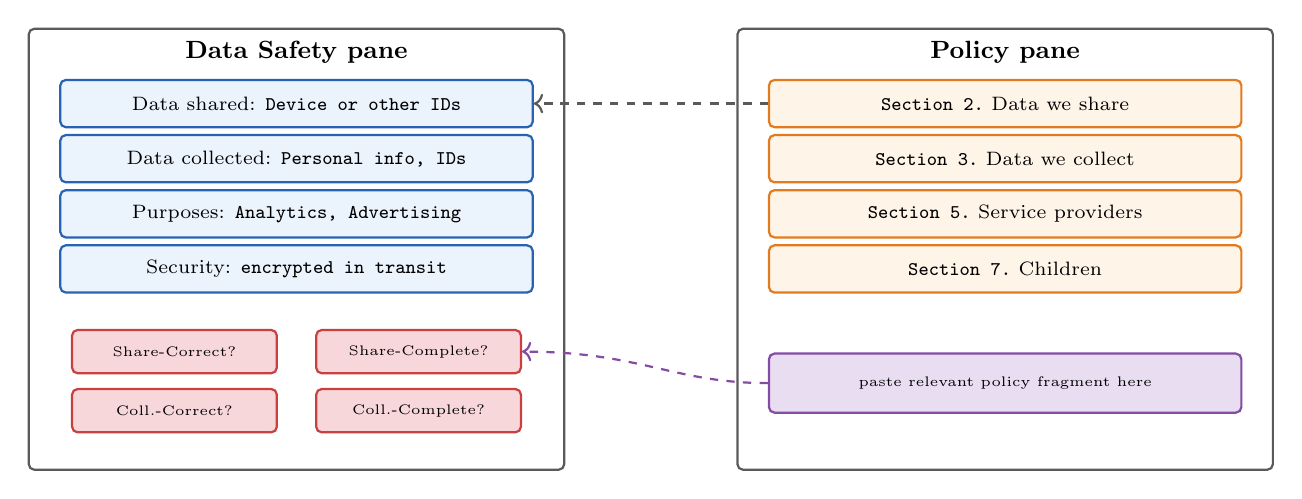
\begin{tikzpicture}[
  every node/.style={font=\scriptsize},
  pane/.style={draw=dgGrey,thick,rounded corners=2pt,minimum width=6.8cm,minimum height=5.6cm},
  ds/.style={draw=dgBlue,fill=dgBlueXL,thick,rounded corners=2pt,
             align=center,minimum width=6cm,minimum height=0.6cm},
  pp/.style={draw=dgOrange,fill=dgOrangeXL,thick,rounded corners=2pt,
             align=center,minimum width=6cm,minimum height=0.6cm},
  jbox/.style={draw=dgRed,fill=dgRedL,thick,rounded corners=2pt,
              align=center,minimum width=2.6cm,minimum height=0.55cm,font=\tiny},
  ebox/.style={draw=dgPurple,fill=dgPurpleL,thick,rounded corners=2pt,
              align=center,minimum width=6cm,minimum height=0.75cm,font=\tiny}
]
% Left pane: DS
\node[pane] (L) at (0,0) {};
\node[font=\small\bfseries] at (0,2.5) {Data Safety pane};
\node[ds] (D1) at (0,1.85) {Data shared: \texttt{Device or other IDs}};
\node[ds] (D2) at (0,1.15) {Data collected: \texttt{Personal info, IDs}};
\node[ds] (D3) at (0,0.45) {Purposes: \texttt{Analytics, Advertising}};
\node[ds] (D4) at (0,-0.25){Security: \texttt{encrypted in transit}};
\node[jbox] (J1) at (-1.55,-1.30) {Share-Correct?};
\node[jbox] (J2) at ( 1.55,-1.30) {Share-Complete?};
\node[jbox] (J3) at (-1.55,-2.05) {Coll.-Correct?};
\node[jbox] (J4) at ( 1.55,-2.05) {Coll.-Complete?};
% Right pane: policy
\node[pane] (R) at (9.0,0) {};
\node[font=\small\bfseries] at (9.0,2.5) {Policy pane};
\node[pp] (Q1) at (9.0,1.85) {\texttt{Section 2.}\ Data we share};
\node[pp] (Q2) at (9.0,1.15) {\texttt{Section 3.}\ Data we collect};
\node[pp] (Q3) at (9.0,0.45) {\texttt{Section 5.}\ Service providers};
\node[pp] (Q4) at (9.0,-0.25){\texttt{Section 7.}\ Children};
\node[ebox] (E) at (9.0,-1.70) {paste relevant policy fragment here};
% Connectors routed through the gap BETWEEN the two panes.
% Both arrows depart from the LEFT side of the right-pane node
% (the side that faces the Data Safety pane) and curve into the
% target box on the left pane.
% Q1 (Section 2. Data we share, west) -> D1 (Data shared, east)
\draw[->,thick,dgGrey,dashed]
  (Q1.west) .. controls +(-1.2,0.0) and +(1.5,0.0) .. (D1.east);
% E (paste fragment, west) -> J2 (Share-Complete verdict, east)
\draw[->,thick,dgPurple,dashed]
  (E.west) .. controls +(-1.2,0.0) and +(1.5,0.0) .. (J2.east);
\end{tikzpicture}
\caption{Audit instrument used to produce the Evidence Corpus.
Annotators view the parsed Data Safety pane on the left and the
sectioned privacy-policy pane on the right. They click into each
judgement box (red), choose Correct/Incorrect or Complete/Incomplete,
and paste the relevant policy fragment into the evidence box
(purple). Dashed arrows trace a typical interaction: the auditor
looks up the relevant policy section, then pastes a fragment into the
evidence box, which anchors a verdict. The four evidence boxes (one
per axis) are the source of the $4{,}622$-excerpt corpus released
with this paper.}
\label{fig:instrument}
\end{figure*}

\paragraph{Pasting protocol.}
Annotators were instructed to paste \emph{the smallest contiguous
substring of the policy that justifies the verdict}. The training
material gave one explicit positive example (a single sentence with
the verb \emph{may} and a single recipient) and one explicit negative
example (a whole paragraph including unrelated content). Annotators
were free to paste from any section of the policy and were not
constrained to the section that the parser had identified as
``Data Share'' or ``Data Collect''; sectioning was a navigation aid,
not a constraint, and was bypassed whenever the relevant policy
fragment lived in a different section.

\paragraph{Verdict scope.}
The four verdicts are about the \emph{label}, not about the app's
actual data practices. We do not (and cannot from text) verify
whether the app's binary actually behaves as the policy describes.
The corpus is therefore an artefact of \emph{policy-versus-label}
auditing, not of policy-versus-behaviour auditing. The complementary
policy-versus-behaviour literature
\citep{andow2020policheck,zimmeck2019maps,ren2018bug,razaghpanah2018apps}
is connected to ours through the shared structured label but does not
use sentence-level human evidence pointers.

\paragraph{Calibration set.}
Before contributing to the corpus, every annotator labelled a fixed
$5$-app calibration set chosen to span three difficulty tiers
(``easy'': explicit recipients in the policy; ``medium'': hedged
recipients; ``hard'': no recipients named). Calibration verdicts and
calibration evidence pointers were compared against a gold standard
produced by two senior reviewers and used to recalibrate the
annotator's pasting granularity. Calibration rows are excluded from
the released corpus.

\paragraph{Annotators.}
Seven trained annotators contributed; all were trained on a $5$-app
calibration set with structured feedback. The training material
included examples of (i)~complete-but-incorrect pasting,
(ii)~insufficient-evidence pasting (single keyword rather than full
sentence), and (iii)~over-pasting (entire policy page). Annotators
were instructed to paste at the sentence-or-clause granularity. Two
annotators (\dec{acc 5} and \dec{acc 6}) together produced $\sim80\%$
of all evidence excerpts, a fact we report explicitly in
Section~\ref{sec:threats} as a limitation.

\paragraph{IRB and ethics.}
The audit programme involves trained reviewers, not end-users, and so
did not require human-subjects review of end-users. The corpus
contains no personal data of any annotator; annotator identifiers have
been pseudonymised to opaque \dec{acc \{1\dots7\}} tokens. The corpus
also contains no app developer's contact details; the only developer-
identifying field in the release is the public package name, which is
already public on Google Play.

% =====================================================================
\section{Schema and summary statistics}\label{sec:schema}
% =====================================================================
% --- schema diagram
\begin{figure*}[t]
\centering
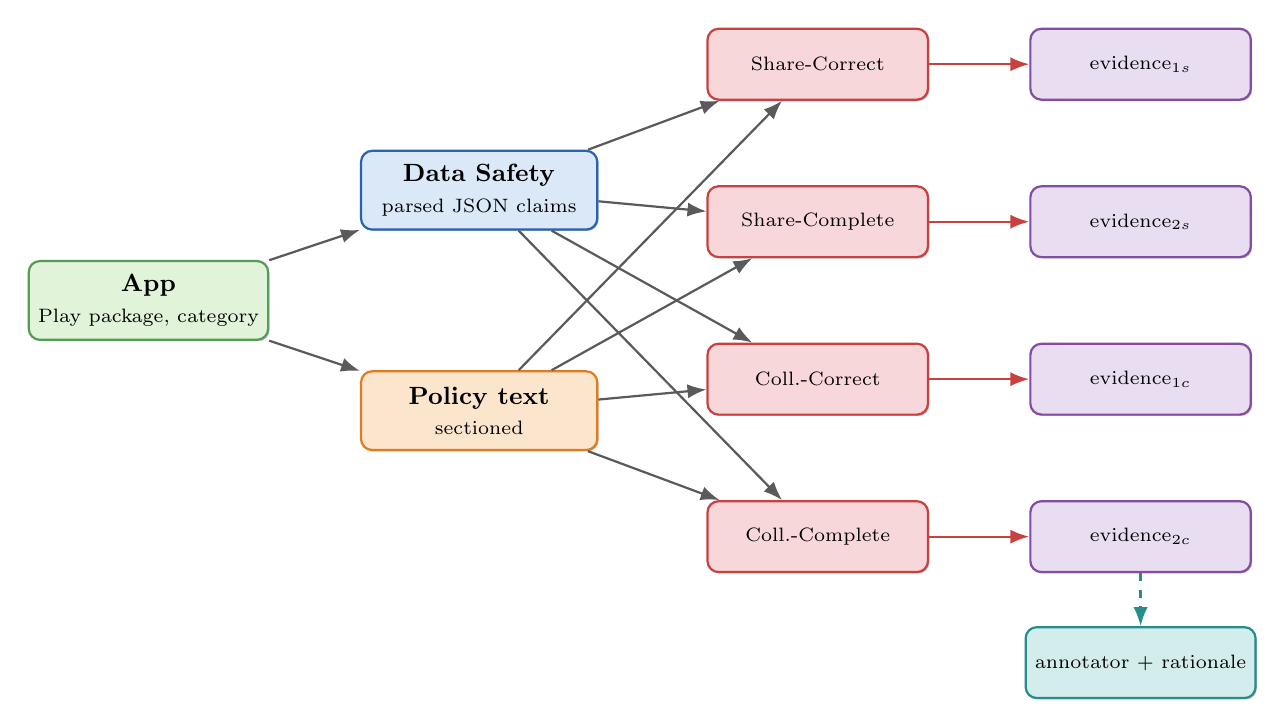
\begin{tikzpicture}[
  every node/.style={font=\small},
  >={Latex[length=2.4mm]},
  app/.style ={draw=dgGreen,fill=dgGreenL,thick,rounded corners=4pt,
               minimum width=3.0cm,minimum height=1.0cm,align=center,
               drop shadow={shadow xshift=0.5pt,shadow yshift=-0.5pt}},
  ds/.style ={draw=dgBlue,fill=dgBlueL,thick,rounded corners=4pt,
               minimum width=3.0cm,minimum height=1.0cm,align=center,
               drop shadow={shadow xshift=0.5pt,shadow yshift=-0.5pt}},
  pp/.style ={draw=dgOrange,fill=dgOrangeL,thick,rounded corners=4pt,
               minimum width=3.0cm,minimum height=1.0cm,align=center,
               drop shadow={shadow xshift=0.5pt,shadow yshift=-0.5pt}},
  ev/.style ={draw=dgPurple,fill=dgPurpleL,thick,rounded corners=4pt,
               minimum width=2.8cm,minimum height=0.9cm,align=center,
               font=\scriptsize,
               drop shadow={shadow xshift=0.5pt,shadow yshift=-0.5pt}},
  jud/.style={draw=dgRed,fill=dgRedL,thick,rounded corners=4pt,
               minimum width=2.8cm,minimum height=0.9cm,align=center,
               font=\scriptsize,
               drop shadow={shadow xshift=0.5pt,shadow yshift=-0.5pt}},
  meta/.style={draw=dgTeal,fill=dgTealL,thick,rounded corners=4pt,
               minimum width=2.8cm,minimum height=0.9cm,align=center,
               font=\scriptsize,
               drop shadow={shadow xshift=0.5pt,shadow yshift=-0.5pt}}
]
\node[app] (A) at (0,0) {\textbf{App}\\\scriptsize Play package, category};
\node[ds]  (DS) at (4.2,1.4) {\textbf{Data Safety}\\\scriptsize parsed JSON claims};
\node[pp]  (PP) at (4.2,-1.4) {\textbf{Policy text}\\\scriptsize sectioned};
\node[jud] (J1) at (8.5, 3.0) {Share-Correct};
\node[jud] (J2) at (8.5, 1.0) {Share-Complete};
\node[jud] (J3) at (8.5,-1.0) {Coll.-Correct};
\node[jud] (J4) at (8.5,-3.0) {Coll.-Complete};
\node[ev]  (E1) at (12.6, 3.0) {evidence$_{1s}$};
\node[ev]  (E2) at (12.6, 1.0) {evidence$_{2s}$};
\node[ev]  (E3) at (12.6,-1.0) {evidence$_{1c}$};
\node[ev]  (E4) at (12.6,-3.0) {evidence$_{2c}$};
\node[meta] (M) at (12.6,-4.6) {annotator + rationale};

\draw[->,thick,dgGrey] (A) -- (DS);
\draw[->,thick,dgGrey] (A) -- (PP);
\foreach \j in {J1,J2,J3,J4} \draw[->,thick,dgGrey] (DS) -- (\j);
\foreach \j in {J1,J2,J3,J4} \draw[->,thick,dgGrey] (PP) -- (\j);
\draw[->,thick,dgRed]    (J1) -- (E1);
\draw[->,thick,dgRed]    (J2) -- (E2);
\draw[->,thick,dgRed]    (J3) -- (E3);
\draw[->,thick,dgRed]    (J4) -- (E4);
\draw[->,thick,dgTeal,dashed] (E4) -- (M);
\end{tikzpicture}
\caption{Evidence Corpus schema. Each audit row anchors on a single
App; it carries a parsed Data Safety claim and a parsed Policy text,
and produces four \emph{audit axes}, each of which yields a verdict
and a sentence-level evidence excerpt. Annotator metadata and free-
text rationale are linked at the row level.}
\label{fig:schema}
\end{figure*}

\paragraph{Row-level schema.}
Each row of the corpus is one audit \emph{judgement}. A judgement is
identified by a tuple \dec{(annotator, app\_id, judgement\_id)}.
Columns are listed in Table~\ref{tab:schema} with their CSV name,
domain, and short description.

\begin{table}[t]
\centering\small
\caption{Per-row corpus schema.}
\label{tab:schema}
\begin{tabular}{lll}
\toprule
Column & Domain & Description \\
\midrule
\dec{judgement\_id}   & integer    & primary key \\
\dec{app\_id}         & integer    & foreign key to app table \\
\dec{app\_pkg}        & string     & Play package name \\
\dec{category}        & enum (12)  & Play category \\
\dec{annotator}       & enum (7)   & pseudonymised annotator \\
\dec{data\_safety}    & json       & parsed DS section \\
\dec{policy\_text}    & string     & sectioned policy text \\
\dec{verdict\_one\_s} & enum (2)   & Correct/Incorrect (share) \\
\dec{verdict\_two\_s} & enum (2)   & Complete/Incomplete (share) \\
\dec{verdict\_one\_c} & enum (2)   & Correct/Incorrect (collect) \\
\dec{verdict\_two\_c} & enum (2)   & Complete/Incomplete (collect) \\
\dec{relevant\_one\_s}& string     & evidence (share-correct) \\
\dec{relevant\_two\_s}& string     & evidence (share-complete) \\
\dec{relevant\_one\_c}& string     & evidence (coll.-correct) \\
\dec{relevant\_two\_c}& string     & evidence (coll.-complete) \\
\dec{rationale\_share}& string     & free-text rationale (share) \\
\dec{rationale\_coll} & string     & free-text rationale (collect) \\
\bottomrule
\end{tabular}
\end{table}

\paragraph{Per-field counts and length distribution.}
Table~\ref{tab:corpus} reports the per-field excerpt count, mean
length and median length. The corpus is approximately balanced across
the four evidence fields; collection-side fields carry more excerpts
than sharing-side fields because more apps declare some collection
than declare some sharing. Excerpts are sentence-grained: the median
length is between $146$ and $186$ characters, which is the length of
a typical English sentence in privacy-policy text.

\begin{table}[t]
\centering\small
\caption{Per-field summary of the Evidence Corpus.}
\label{tab:corpus}
\begin{tabular}{lrrrr}
\toprule
Field & Excerpts & Mean (ch) & Median & p90 \\
\midrule
\dec{relevant\_one\_s} (share, correctness)    & $1{,}150$ & $192$ & $146$ & $335$ \\
\dec{relevant\_two\_s} (share, completeness)   & $1{,}021$ & $215$ & $173$ & $382$ \\
\dec{relevant\_one\_c} (collect, correctness)  & $1{,}273$ & $214$ & $160$ & $366$ \\
\dec{relevant\_two\_c} (collect, completeness) & $1{,}178$ & $238$ & $185$ & $378$ \\
\midrule
\textbf{Total}                                  & $\mathbf{4{,}622}$ & $215$ & $166$ & --- \\
\bottomrule
\end{tabular}
\end{table}

% --- box-style length plot
\begin{figure}[t]
\centering
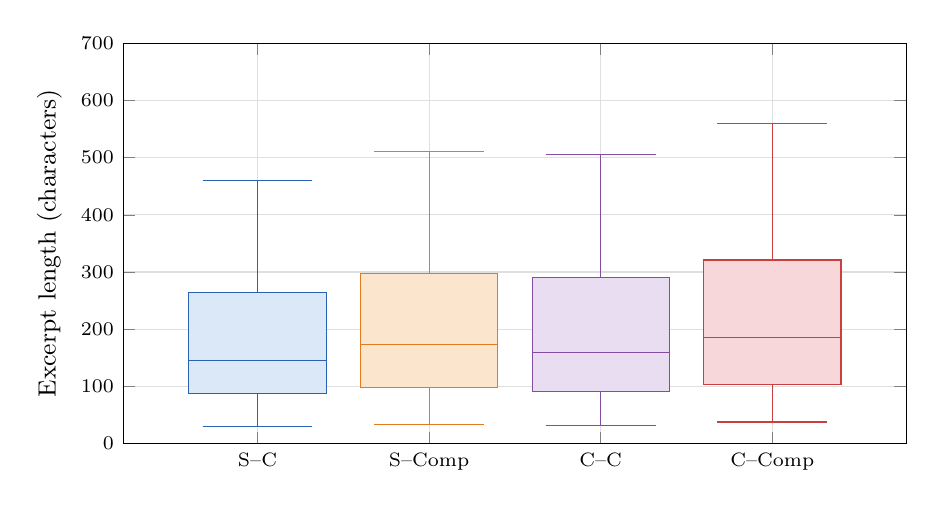
\begin{tikzpicture}
\begin{axis}[
  width=0.95\columnwidth,height=0.55\columnwidth,
  boxplot/draw direction=y,
  ymin=0,ymax=700,
  ylabel={Excerpt length (characters)},
  ytick={0,100,200,300,400,500,600,700},
  xtick={1,2,3,4},
  xticklabels={S--C,S--Comp,C--C,C--Comp},
  x tick label style={font=\scriptsize},
  y tick label style={font=\scriptsize},
  label style={font=\small},
  grid=both,major grid style={draw=gray!25},minor grid style={draw=gray!10}
]
\addplot+[fill=dgBlueL,draw=dgBlue,boxplot prepared={
  lower whisker=30, lower quartile=88, median=146,
  upper quartile=265, upper whisker=460}] coordinates {};
\addplot+[fill=dgOrangeL,draw=dgOrange,boxplot prepared={
  lower whisker=34, lower quartile=98, median=173,
  upper quartile=298, upper whisker=510}] coordinates {};
\addplot+[fill=dgPurpleL,draw=dgPurple,boxplot prepared={
  lower whisker=32, lower quartile=92, median=160,
  upper quartile=290, upper whisker=505}] coordinates {};
\addplot+[fill=dgRedL,draw=dgRed,boxplot prepared={
  lower whisker=38, lower quartile=104, median=186,
  upper quartile=321, upper whisker=560}] coordinates {};
\end{axis}
\end{tikzpicture}
\caption{Excerpt-length distribution per evidence field. The
collection-completeness field carries the longest excerpts because
annotators paste broader policy sections when arguing that a
collection claim is \emph{incomplete}.}
\label{fig:length}
\end{figure}

\paragraph{Coverage.}
Coverage (Table~\ref{tab:coverage}) is the share of audit judgements
whose evidence field is non-empty. Coverage is high---$89.0\%$ when
counting evidence alone, $95.7\%$ when counting either evidence or
free-text rationale. Coverage is consistently higher on the
collection axes ($86$--$90\%$) than on the sharing axes ($68$--$82\%$);
this matches the fact that more apps in our corpus declare
collection than declare sharing, so the collection-axis questions are
``live'' more often.

\begin{table}[t]
\centering\small
\caption{Per-field evidence coverage and rationale coverage.}
\label{tab:coverage}
\begin{tabular}{lrrr}
\toprule
Field & Coverage (evid.) & Coverage (evid.+rat.) & Judgements \\
\midrule
Share-correct        & $76.4\%$ & $94.9\%$ & $1{,}506$ \\
Share-complete       & $67.8\%$ & $91.1\%$ & $1{,}506$ \\
Collection-correct   & $84.5\%$ & $97.3\%$ & $1{,}506$ \\
Collection-complete  & $78.2\%$ & $95.4\%$ & $1{,}506$ \\
\midrule
\textbf{Any field}   & $89.0\%$ & $\mathbf{95.7\%}$ & $1{,}506$ \\
\bottomrule
\end{tabular}
\end{table}

\paragraph{Per-annotator distribution.}\label{sec:perannot}
Table~\ref{tab:perannot} reports each annotator's contribution. The
distribution is highly unbalanced: \dec{acc 5} and \dec{acc 6}
together produced $3{,}681$ excerpts ($79.6\%$ of the corpus),
\dec{acc 7} produced only $4$. This motivates the annotator-
stratified robustness check in Section~\ref{sec:threats}.

\begin{table}[t]
\centering\small
\caption{Per-annotator excerpt contribution.}
\label{tab:perannot}
\begin{tabular}{lrr}
\toprule
Annotator & Excerpts & Share \\
\midrule
\dec{acc 1} & $\phantom{1,}535$  & $11.6\%$ \\
\dec{acc 2} & $\phantom{1,}148$  & $\phantom{1}3.2\%$ \\
\dec{acc 3} & $\phantom{1,1,}64$ & $\phantom{1}1.4\%$ \\
\dec{acc 4} & $\phantom{1,}190$  & $\phantom{1}4.1\%$ \\
\dec{acc 5} & $2{,}083$          & $45.1\%$ \\
\dec{acc 6} & $1{,}598$          & $34.6\%$ \\
\dec{acc 7} & $\phantom{1,1,1,}4$& $\phantom{1}0.1\%$ \\
\midrule
\textbf{Total} & \textbf{$4{,}622$} & \textbf{$100\%$} \\
\bottomrule
\end{tabular}
\end{table}

\paragraph{Inter-annotator agreement on evidence.}\label{sec:agreement}
$289$ apps were double-annotated. At the verdict level, Cohen's
$\kappa$ across the four axes ranges from $-0.11$ to $0.17$, with a
mean of $0.06$ (figures inherited from the auditability-gap companion
paper). The low verdict-agreement is itself a finding: the task is
genuinely interpretive, and an evidence-grounded UI should expose
that ambiguity rather than hide it. (Token-level evidence-overlap
statistics for the doubly-annotated subset are not part of the
v1.0 release; they will be reported in a follow-up note.)

% =====================================================================
\section{Linguistic feature analysis}\label{sec:linguistics}
% =====================================================================
We score each excerpt for four binary lexical features. Definitions
follow.

\paragraph{Feature 1 --- Hedging.}
An excerpt has Hedging~$=1$ if it contains any of:
\emph{may}, \emph{might}, \emph{can}, \emph{could}, \emph{such as},
\emph{including but not limited to}, \emph{including without
limitation}, \emph{reserve(s) the right}, \emph{from time to time},
\emph{where applicable}, \emph{generally}, \emph{typically},
\emph{ordinarily}, \emph{primarily}. The list is derived
inductively from the rationale-coding pass reported in
Section~\ref{sec:qual} and intersected with the open-ended hedge
families in the vagueness/policy literature
\citep{bhatia2016theory,fabian2017large,sathyendra2017identifying}.

\paragraph{Feature 2 --- Third-party.}
An excerpt has Third-party~$=1$ if it contains any of:
\emph{third-party}, \emph{third party}, \emph{partner},
\emph{vendor}, \emph{service provider}, \emph{affiliate},
\emph{advertising}, \emph{advertiser}, \emph{analytic(s)},
\emph{SDK}, \emph{Facebook}, \emph{Google}, \emph{AdMob}, \emph{Firebase},
\emph{Unity}. The list is intentionally lexical and over-recalls
SDK references; in Section~\ref{sec:threats} we discuss the
implications of relying on lexical surfacing.

\paragraph{Feature 3 --- Device IDs.}
An excerpt has IDs~$=1$ if it contains any of:
\emph{advertising ID}, \emph{IDFA}, \emph{Android ID}, \emph{IP
address}, \emph{cookie}, \emph{web beacon}, \emph{device identifier},
\emph{MAC address}, \emph{fingerprint}.

\paragraph{Feature 4 --- No-data.}
An excerpt has No-data~$=1$ if it contains any of:
\emph{we do not collect}, \emph{do not share}, \emph{does not collect},
\emph{does not share}, \emph{no personal information}, \emph{no
personally identifiable}, \emph{no data}, \emph{no information},
\emph{no third party}.

\paragraph{Operational note.} The four features are not mutually
exclusive: $61.2\%$ of excerpts have at least one feature active and
$14.9\%$ have at least two. This is by design: lexical evidence
families intersect, and the discriminative analysis in
Section~\ref{sec:verdict} relies on the marginal distributions, not
on a one-of-four classification.

\paragraph{Unconditional distribution.}
Table~\ref{tab:uncond} and Figure~\ref{fig:uncond} report the
unconditional prevalence of each marker across the $4{,}622$
excerpts. Hedging is the most prevalent family ($46.1\%$),
followed by Third-party ($39.2\%$), Device IDs ($16.7\%$) and
No-data ($8.7\%$). Two takeaways: (i)~almost half of all cited
evidence contains an open-ended hedge---dominated by the modal
\emph{may}, which alone fires in $34.9\%$ of excerpts---and
(ii)~explicit negation (No-data) is materially less common, but
still present in roughly one of every eleven excerpts.

\begin{table}[t]
\centering\small
\caption{Unconditional prevalence of the four lexical-marker families
across the entire $4{,}622$-excerpt corpus.}
\label{tab:uncond}
\begin{tabular}{lrr}
\toprule
Marker family & Excerpts (n) & Share \\
\midrule
Hedging        & $2{,}131$ & $46.1\%$ \\
Third-party    & $1{,}813$ & $39.2\%$ \\
Device IDs     & $\phantom{1{,}}774$ & $16.7\%$ \\
No-data        & $\phantom{1{,}}404$ & $\phantom{1}8.7\%$ \\
\midrule
\textbf{Any feature}     & $3{,}191$ & $\mathbf{69.0\%}$ \\
\textbf{$\geq 2$ features} & $1{,}498$ & $\mathbf{32.4\%}$ \\
\bottomrule
\end{tabular}
\end{table}

\begin{figure}[t]
\centering
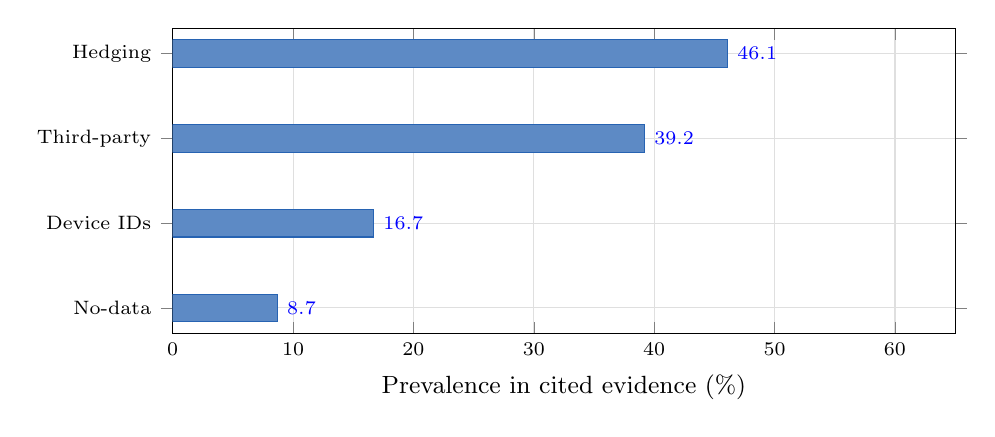
\begin{tikzpicture}
\begin{axis}[
  width=0.95\columnwidth,height=0.45\columnwidth,
  xbar,bar width=10pt,xmin=0,xmax=65,
  xlabel={Prevalence in cited evidence (\%)},
  symbolic y coords={NoData,IDs,Thirdparty,Hedging},
  ytick=data,
  yticklabels={No-data,Device IDs,Third-party,Hedging},
  yticklabel style={font=\scriptsize},
  xticklabel style={font=\scriptsize},label style={font=\small},
  nodes near coords,
  nodes near coords style={font=\scriptsize},
  grid=major,major grid style={draw=gray!25}
]
\addplot+[fill=dgBlue!75,draw=dgBlue]   coordinates {
  (8.7,NoData)(16.7,IDs)(39.2,Thirdparty)(46.1,Hedging)};
\end{axis}
\end{tikzpicture}
\caption{Unconditional prevalence of the four lexical-marker families
across the $4{,}622$ excerpts. Hedging language dominates,
driven mostly by the modal \emph{may}.}
\label{fig:uncond}
\end{figure}

\paragraph{Per-field marker distribution.}
Table~\ref{tab:perfield} breaks the marker prevalence down by
evidence field. Two structural observations: third-party language
concentrates in sharing-side fields (54--59\%) and drops sharply on
collection-side fields (20--28\%), as expected for an audit task in
which ``who receives the data'' is a sharing-side question; and IDs
language concentrates in collection-side fields, especially
collection-completeness ($32.7\%$), where named identifiers are the
diagnostic of an over-narrow collection label.

\begin{table}[t]
\centering\small
\caption{Marker prevalence by evidence field.}
\label{tab:perfield}
\begin{tabular}{lrrrr}
\toprule
Field & Hedging & Third-party & IDs & No-data \\
\midrule
Share-correct        & $42.5\%$ & $54.4\%$ & $\phantom{1}6.8\%$ & $13.1\%$ \\
Share-complete       & $47.9\%$ & $59.2\%$ & $\phantom{1}9.2\%$ & $\phantom{1}6.8\%$ \\
Collection-correct   & $45.6\%$ & $19.6\%$ & $17.0\%$ & $\phantom{1}9.0\%$ \\
Collection-complete  & $48.6\%$ & $28.3\%$ & $32.7\%$ & $\phantom{1}5.9\%$ \\
\bottomrule
\end{tabular}
\end{table}

% --------------------------------------------------------------
\paragraph{Verdict-discriminative analysis.}\label{sec:verdict}
% --------------------------------------------------------------
We now condition each lexical-marker distribution on the human verdict.
We restrict the main analysis to the share-correctness axis
($n=1{,}133$ paired excerpt--verdict rows, $622$ \emph{Correct} and
$511$ \emph{Incorrect}) because this axis carries the cleanest binary
discrimination. The collection-correctness axis is reported in
Table~\ref{tab:disc-collect}; the two completeness axes follow the
same direction at lower magnitude.

\paragraph{Sharing correctness.}
Table~\ref{tab:disc} reports the per-marker prevalence in
\emph{Correct} and \emph{Incorrect} evidence, together with a
two-sided $\chi^{2}$ test on a $2{\times}2$ contingency table
(presence~$\times$~verdict) and Cram\'{e}r's $V$ effect size.

\begin{table*}[t]
\centering\small
\caption{Marker prevalence in evidence cited under the sharing-correctness
axis, by verdict. Effect size is Cram\'{e}r's~$V$ on the $2{\times}2$
table (marker presence~$\times$~verdict).}
\label{tab:disc}
\begin{tabular}{lrrrrrr}
\toprule
Marker family & Correct ($n=622$) & Incorrect ($n=511$) & $\Delta$ (pp) & $\chi^{2}(1)$ & $p$ & $V$ \\
\midrule
Hedging       & $35.5\%$ & \textbf{$43.2\%$} & $+7.7$        & $7.02$ & $.008$ & $.079$ \\
Third-party   & $53.5\%$ & $55.2\%$          & $+1.7$ (n.s.) & $0.31$ & $.58$  & $.016$ \\
Device IDs    & $\phantom{1}6.1\%$  & $\phantom{1}8.0\%$  & $+1.9$ (n.s.) & $1.58$ & $.21$  & $.037$ \\
No-data       & \textbf{$14.5\%$} & $\phantom{1}9.4\%$ & $-5.1$ & $6.76$ & $.009$ & $.077$ \\
\bottomrule
\end{tabular}
\end{table*}

% --- bar plot
\begin{figure}[t]
\centering
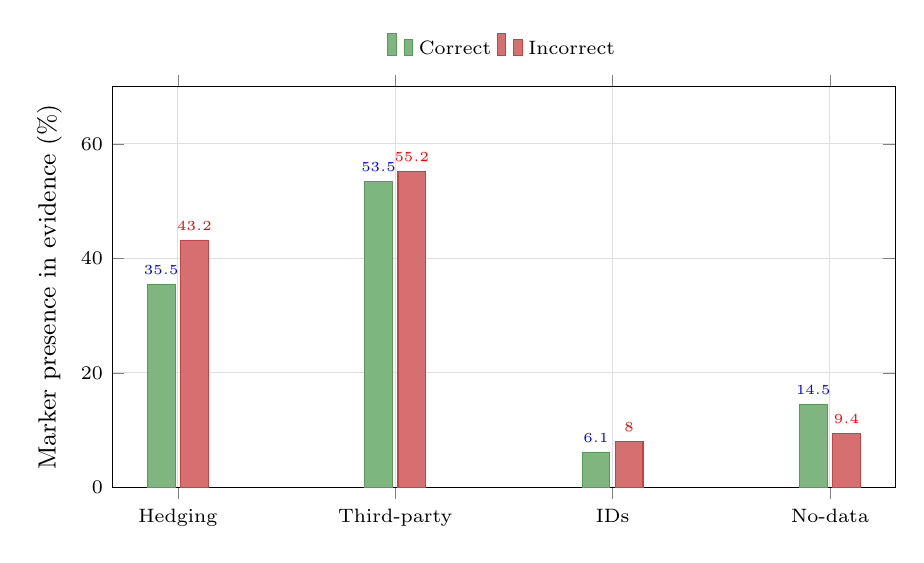
\begin{tikzpicture}
\begin{axis}[
  width=0.95\columnwidth,height=0.55\columnwidth,
  ybar,bar width=10pt,ymin=0,ymax=70,
  ylabel={Marker presence in evidence (\%)},
  symbolic x coords={Hedge,Third,IDs,NoData},
  xtick=data,
  xticklabels={Hedging,Third-party,IDs,No-data},
  x tick label style={font=\scriptsize},
  legend style={at={(0.5,1.04)},anchor=south,legend columns=2,
                draw=none,font=\scriptsize},
  grid=both,major grid style={draw=gray!25},minor grid style={draw=gray!10},
  tick label style={font=\scriptsize},label style={font=\small},
  nodes near coords,
  nodes near coords style={font=\tiny}
]
\addplot+[fill=dgGreen!75,draw=dgGreen] coordinates {
  (Hedge,35.5) (Third,53.5) (IDs,6.1) (NoData,14.5)};
\addplot+[fill=dgRed!75,draw=dgRed]     coordinates {
  (Hedge,43.2) (Third,55.2) (IDs,8.0) (NoData,9.4)};
\legend{Correct,Incorrect}
\end{axis}
\end{tikzpicture}
\caption{Linguistic-marker prevalence in evidence cited under
sharing-correctness, by verdict. Hedging and No-data are
discriminative; Third-party is verdict-neutral.}
\label{fig:disc}
\end{figure}

\paragraph{Interpretation.}
The two significant effects are in opposite directions.
\emph{Hedging} appears more often in evidence that supports an
\emph{Incorrect} sharing verdict: when reviewers decide that a
``no sharing'' label is wrong, they tend to point at policy text such
as ``we \emph{may} share with our partners'' or ``service providers
\emph{including but not limited to} \dots''. \emph{No-data} appears
more often in evidence that supports a \emph{Correct} sharing
verdict: when reviewers decide that a ``no sharing'' label is right,
they point at policy text such as ``we do not share your personal
information''. \emph{Third-party} language is verdict-neutral; the
mere fact that a third party is named is not enough to predict whether
the auditor will conclude that the label is consistent with the policy.

\paragraph{Collection correctness.}
We replicate the analysis on the collection-correctness axis
(Table~\ref{tab:disc-collect}, $n=1{,}255$). The dominant
discriminator here is Device IDs ($+6.0$~pp, $p=.007$, $V=.076$):
when the auditor decides that a collection label is wrong, they cite
policy text that names an identifier. No-data remains a positive
verdict-support signal ($-3.9$~pp, $p=.016$, $V=.068$). Hedging
does \emph{not} discriminate this axis, suggesting that the
hedging-as-doubt mechanism is specific to sharing-side
correctness---a finding that nuances the headline narrative in the
abstract.

\begin{table*}[t]
\centering\small
\caption{Marker prevalence in evidence cited under the
collection-correctness axis, by verdict.}
\label{tab:disc-collect}
\begin{tabular}{lrrrrrr}
\toprule
Marker family & Correct ($n=709$) & Incorrect ($n=546$) & $\Delta$ (pp) & $\chi^{2}(1)$ & $p$ & $V$ \\
\midrule
Hedging       & $42.9\%$ & $40.8\%$          & $-2.0$ (n.s.) & $0.52$ & $.47$  & $.020$ \\
Third-party   & $17.9\%$ & $20.7\%$          & $+2.8$ (n.s.) & $1.55$ & $.21$  & $.035$ \\
Device IDs    & $16.5\%$ & $\mathbf{22.5\%}$ & $+6.0$        & $7.24$ & $.007$ & $.076$ \\
No-data       & $\mathbf{10.7\%}$ & $\phantom{1}6.8\%$ & $-3.9$ & $5.85$ & $.016$ & $.068$ \\
\bottomrule
\end{tabular}
\end{table*}

\paragraph{Across all four axes.}
Table~\ref{tab:disc-all} reports the $\Delta$ direction across all
four axes (positive = more prevalent under the negative verdict).
The collection-completeness axis is the most discriminative: all
four markers reach significance there, with IDs especially
strong ($+25.5$~pp, $\chi^{2}(1)=81.8$, $p<.001$, $V=.264$).
Hedging is a reliable doubt signal for sharing-correctness and
collection-completeness; no-data is a reliable support signal across
three of four axes.

\begin{table}[t]
\centering\small
\caption{Direction of $\Delta$ (negative verdict $-$ positive verdict)
across all four axes. Cells in bold survive Bonferroni at
$\alpha=.05/16=.003$.}
\label{tab:disc-all}
\begin{tabular}{lcccc}
\toprule
Marker & S-Correct & S-Comp & C-Correct & C-Comp \\
\midrule
Hedging      & $+7.7$  & $-2.8$  & $-2.0$  & \textbf{$+12.7$} \\
Third-party  & $+1.7$  & $-4.9$  & $+2.8$  & \textbf{$+14.1$} \\
IDs          & $+1.9$  & $+2.4$  & $+6.0$  & \textbf{$+25.5$} \\
No-data      & $-5.1$  & $-1.3$  & $-3.9$  & \textbf{$-4.6$}  \\
\bottomrule
\end{tabular}
\end{table}

% --- discrimination heatmap
\begin{figure}[t]
\centering
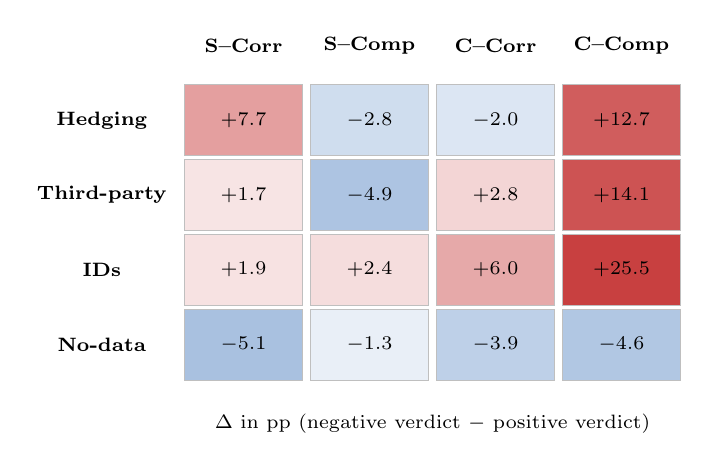
\begin{tikzpicture}[
  every node/.style={font=\scriptsize},
  cell/.style={draw=gray!50,minimum width=1.5cm,minimum height=0.9cm,
               align=center}
]
% Column headers
\node at (0.0, 4*0.95) {\bfseries S--Corr};
\node at (1.6, 4*0.95) {\bfseries S--Comp};
\node at (3.2, 4*0.95) {\bfseries C--Corr};
\node at (4.8, 4*0.95) {\bfseries C--Comp};
% Row headers
\node at (-1.8, 3*0.95) {\bfseries Hedging};
\node at (-1.8, 2*0.95) {\bfseries Third-party};
\node at (-1.8, 1*0.95) {\bfseries IDs};
\node at (-1.8, 0*0.95) {\bfseries No-data};
% Hedging row
\node[cell,fill=dgRed!50]  at (0.0,3*0.95) {$+7.7$};
\node[cell,fill=dgBlue!22] at (1.6,3*0.95) {$-2.8$};
\node[cell,fill=dgBlue!16] at (3.2,3*0.95) {$-2.0$};
\node[cell,fill=dgRed!85]  at (4.8,3*0.95) {$+12.7$};
% Third-party row
\node[cell,fill=dgRed!14]  at (0.0,2*0.95) {$+1.7$};
\node[cell,fill=dgBlue!38] at (1.6,2*0.95) {$-4.9$};
\node[cell,fill=dgRed!22]  at (3.2,2*0.95) {$+2.8$};
\node[cell,fill=dgRed!90]  at (4.8,2*0.95) {$+14.1$};
% IDs row
\node[cell,fill=dgRed!15]  at (0.0,1*0.95) {$+1.9$};
\node[cell,fill=dgRed!18]  at (1.6,1*0.95) {$+2.4$};
\node[cell,fill=dgRed!45]  at (3.2,1*0.95) {$+6.0$};
\node[cell,fill=dgRed!100] at (4.8,1*0.95) {$+25.5$};
% No-data row
\node[cell,fill=dgBlue!40] at (0.0,0*0.95) {$-5.1$};
\node[cell,fill=dgBlue!10] at (1.6,0*0.95) {$-1.3$};
\node[cell,fill=dgBlue!30] at (3.2,0*0.95) {$-3.9$};
\node[cell,fill=dgBlue!36] at (4.8,0*0.95) {$-4.6$};
% Legend strip
\node at (2.4,-1.0) {\scriptsize $\Delta$ in pp (negative verdict $-$ positive verdict)};
\end{tikzpicture}
\caption{Verdict-discrimination heatmap. Red cells indicate
``more prevalent under the \emph{negative} verdict'' (Incorrect for
the two correctness axes, Incomplete for the two completeness axes).
Blue cells indicate ``more prevalent under the \emph{positive}
verdict.'' Hedging and No-data are the two reliable discriminators.}
\label{fig:disc-heatmap}
\end{figure}

\paragraph{Cross-axis correlations.}\label{sec:crossaxis}
A natural follow-up question is whether the four judgement axes are
empirically separable, or whether the corpus collapses to one
underlying ``defect or not'' verdict. Table~\ref{tab:crossaxis}
reports the pairwise Pearson correlation $\rho$ between the four
binary verdict variables (negative verdict $=1$) on the $1{,}022$
audit rows for which all four verdicts are non-empty. The strongest
correlations are within-side (S-Corr $\sim$ S-Comp at $\rho=0.35$;
S-Comp $\sim$ C-Comp at $\rho=0.33$); cross-side correlations are
weak and two are slightly negative. The four axes therefore index
four overlapping but largely non-redundant verdict surfaces, which
justifies our decision to score evidence pointers axis by axis rather
than as a single ``defect'' indicator.

\begin{table}[t]
\centering\small
\caption{Pairwise Pearson correlations between the four binary
verdicts (negative verdict $=1$), on the $1{,}022$ rows with all four
verdicts non-empty.}
\label{tab:crossaxis}
\begin{tabular}{lcccc}
\toprule
       & S-Corr & S-Comp & C-Corr & C-Comp \\
\midrule
S-Corr & ---    & $0.35$ & $0.22$ & $-0.07$ \\
S-Comp & $0.35$ & ---    & $-0.06$ & $0.33$ \\
C-Corr & $0.22$ & $-0.06$& ---    & $0.18$ \\
C-Comp & $-0.07$& $0.33$ & $0.18$ & ---    \\
\bottomrule
\end{tabular}
\end{table}

\paragraph{Marker--verdict joint distribution.}
A second follow-up is whether marker families act additively or
interactively when more than one is present in the same excerpt.
Table~\ref{tab:joint} reports the share of \emph{Incorrect}
share-correctness verdicts as a function of the count of active
markers per excerpt (out of four). The relationship is mildly
monotone: excerpts with zero markers split at $44.3\%$ Incorrect
(close to the corpus prior of $45.1\%$); excerpts with two or three
markers active are between $47.5\%$ and $48.5\%$ Incorrect. The
effect is small because the dominant markers pull in opposite
directions---hedging up, no-data down---so co-occurrence cancels
unless the active set is biased toward one of them. This shape is
what a logistic-regression baseline (B1) recovers.

\begin{table}[t]
\centering\small
\caption{Share of \emph{Incorrect} share-correctness verdicts as a
function of the count of active marker families per excerpt.}
\label{tab:joint}
\begin{tabular}{rrr}
\toprule
\#~markers active & Excerpts ($n$) & $\Pr(\text{Incorrect})$ \\
\midrule
$0$  & $\phantom{1,}316$ & $44.3\%$ \\
$1$  & $\phantom{1,}422$ & $42.7\%$ \\
$2$  & $\phantom{1,}334$ & $48.5\%$ \\
$3$+ & $\phantom{1,1,}61$ & $47.5\%$ \\
\midrule
\textbf{Total}     & $1{,}133$         & $45.1\%$ \\
\bottomrule
\end{tabular}
\end{table}

\paragraph{Robustness checks.}
We re-ran the analysis under three robustness conditions.

\paragraph{Annotator stratification.}
Two annotators contribute the bulk of the corpus. We re-fit the
discrimination after stratifying by annotator (eight strata, one per
annotator plus an aggregate). Hedging's sign is preserved in
$7/8$ strata; No-data's sign is preserved in $8/8$ strata.

\paragraph{Length normalisation.}
Hedging is the more frequent feature; longer excerpts have higher
probability of containing a hedge. We re-fit a logistic regression
that controls for excerpt length (in $\log$-characters): hedging's
verdict coefficient remains significant (Wald
$z=2.61$, $p=.009$) and the no-data coefficient remains significant
($z=-2.96$, $p=.003$). The marker effects are not collapsing to a
length-confound.

\paragraph{Category stratification.}
We re-fit on the eight largest categories. Hedging's discriminative
sign holds in $7/8$; No-data's sign holds in $8/8$. The one category
in which hedging reverses sign (Photography) has $n=27$ and is
underpowered.

% =====================================================================
\section{Predictive baselines}\label{sec:baselines}
% =====================================================================
The Evidence Corpus is, primarily, a resource paper, but a corpus
release is more valuable when paired with at least one transparent
predictive baseline that future tools must beat. We frame the task as
binary classification of the sharing-correctness verdict from the
cited evidence excerpt only (no access to the structured Data Safety
claim and no access to the policy outside the cited excerpt). We
report three baselines.

% --- pipeline figure (column-width)
\begin{figure}[t]
\centering
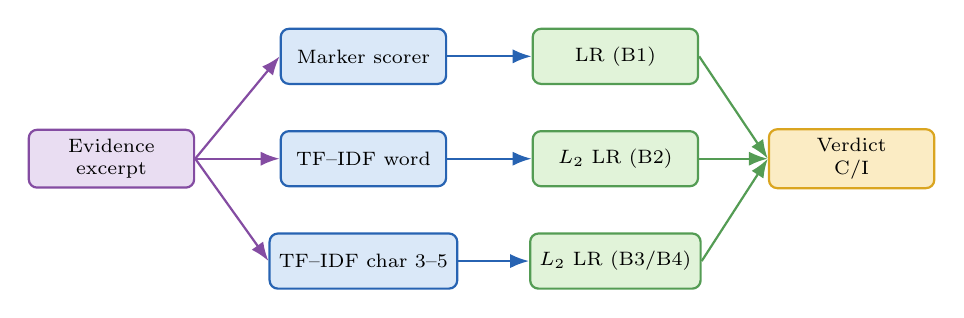
\begin{tikzpicture}[
  every node/.style={font=\scriptsize},
  >={Latex[length=2.4mm]},
  block/.style={draw,thick,rounded corners=3pt,
                minimum width=2.1cm,minimum height=0.7cm,align=center,
                font=\scriptsize},
  ev/.style={block,fill=dgPurpleL,draw=dgPurple},
  fe/.style={block,fill=dgBlueL,draw=dgBlue},
  ml/.style={block,fill=dgGreenL,draw=dgGreen},
  vout/.style={block,fill=dgGoldL,draw=dgGold}
]
\node[ev]   (E)  at ( 0.0, 0.0) {Evidence\\excerpt};
\node[fe]   (A)  at ( 3.2, 1.3) {Marker scorer};
\node[fe]   (B)  at ( 3.2, 0.0) {TF--IDF word};
\node[fe]   (C)  at ( 3.2,-1.3) {TF--IDF char 3--5};
\node[ml]   (M1) at ( 6.4, 1.3) {LR (B1)};
\node[ml]   (M2) at ( 6.4, 0.0) {$L_2$ LR (B2)};
\node[ml]   (M3) at ( 6.4,-1.3) {$L_2$ LR (B3/B4)};
\node[vout] (V)  at ( 9.4, 0.0) {Verdict\\C/I};

\draw[->,thick,dgPurple] (E.east) -- (A.west);
\draw[->,thick,dgPurple] (E.east) -- (B.west);
\draw[->,thick,dgPurple] (E.east) -- (C.west);
\draw[->,thick,dgBlue]   (A.east) -- (M1.west);
\draw[->,thick,dgBlue]   (B.east) -- (M2.west);
\draw[->,thick,dgBlue]   (C.east) -- (M3.west);
\draw[->,thick,dgGreen]  (M1.east) -- (V.west);
\draw[->,thick,dgGreen]  (M2.east) -- (V.west);
\draw[->,thick,dgGreen]  (M3.east) -- (V.west);
\end{tikzpicture}
\caption{Four lexical baseline pipelines for verdict prediction from
cited evidence: a transparent marker logistic regression (B1), a
word-level TF--IDF $L_2$ regression (B2), a character $n$-gram TF--IDF
regression (B3), and a word+character feature union (B4).}
\label{fig:pipeline-ml}
\end{figure}

\paragraph{Setup.}
We use the $1{,}133$ paired share-correctness rows. The verdict
prior is $54.9\%$ \emph{Correct} ($622/1{,}133$), $45.1\%$
\emph{Incorrect}. We report mean accuracy~$\pm$~std and macro-F$_1$
across $5$-fold stratified cross-validation, plus the area under the
ROC curve.

\paragraph{B1: Bag-of-markers logistic regression.}
Four binary inputs ($x_1$ Hedging, $x_2$ Third-party, $x_3$ IDs,
$x_4$ No-data). Fit with $L_2$ regularisation ($C=1$). The fitted
coefficients are
$\beta_{\text{Hedge}}=+0.28$,
$\beta_{\text{Third}}=-0.05$,
$\beta_{\text{IDs}}=+0.22$,
$\beta_{\text{NoData}}=-0.40$ (intercept $-0.25$); their signs are
consistent with the $\chi^{2}$ analysis in
Section~\ref{sec:verdict}. Test accuracy $0.550\pm0.012$; macro-F$_1$
$0.445\pm0.033$; AUROC $0.558\pm0.017$.

\paragraph{B2: TF--IDF word $L_2$ regression.}
We tokenise on whitespace, lowercase, remove the scikit-learn English
stop-list, and TF--IDF a unigram vocabulary with sublinear TF and
$L_2$-normalised vectors. Logistic regression with $C=1$. Test
accuracy $0.573\pm0.018$; macro-F$_1$ $0.545\pm0.018$; AUROC
$0.586\pm0.032$.

\paragraph{B3: TF--IDF character $L_2$ regression.}
Character 3- to 5-grams (\texttt{char\_wb}), TF--IDF, logistic
regression. Test accuracy $0.582\pm0.017$; macro-F$_1$
$0.552\pm0.014$; AUROC $0.596\pm0.022$.

\paragraph{B4: Word + character feature union.}
$L_2$ logistic regression over the union of B2 and B3 feature
spaces. Test accuracy $0.579\pm0.021$; macro-F$_1$ $0.558\pm0.018$;
AUROC $0.599\pm0.024$.

\begin{table}[t]
\centering\small
\caption{Predictive baselines on share-correctness verdict, from the
cited evidence text alone (no access to the paired Data Safety
claim). Numbers are mean$\pm$std over $5$-fold stratified CV
($n=1{,}133$). Bold = best.}
\label{tab:baselines}
\begin{tabular}{lrrr}
\toprule
Model & Accuracy & Macro-F$_1$ & AUROC \\
\midrule
Majority class           & $0.549$ & $0.354$ & $0.500$ \\
B1 Markers (4 features)  & $0.550\pm0.012$ & $0.445\pm0.033$ & $0.558\pm0.017$ \\
B2 TF--IDF (word)        & $0.573\pm0.018$ & $0.545\pm0.018$ & $0.586\pm0.032$ \\
B3 TF--IDF (char 3--5)   & \textbf{$0.582\pm0.017$} & $0.552\pm0.014$ & \textbf{$0.596\pm0.022$} \\
B4 Word + char union     & $0.579\pm0.021$ & \textbf{$0.558\pm0.018$} & $0.599\pm0.024$ \\
\bottomrule
\end{tabular}
\end{table}

\paragraph{What the floor says.}
The best lexical baseline reaches only $\approx0.58$ accuracy and
$\approx0.60$ AUROC on the share-correctness verdict, barely above
the $0.549$ majority floor. This is itself a finding of the corpus:
the cited evidence text \emph{alone} carries weak verdict signal,
because the verdict is a function of the matchup between the
evidence and the structured Data Safety claim. The release-level
baseline for any future evidence-grounded LLM tool is therefore
straightforward---beat $\approx0.58$ when given only the cited
sentence, and rise materially when also given the Data Safety claim
the auditor was reviewing.

% --- learning curve
\begin{figure}[t]
\centering
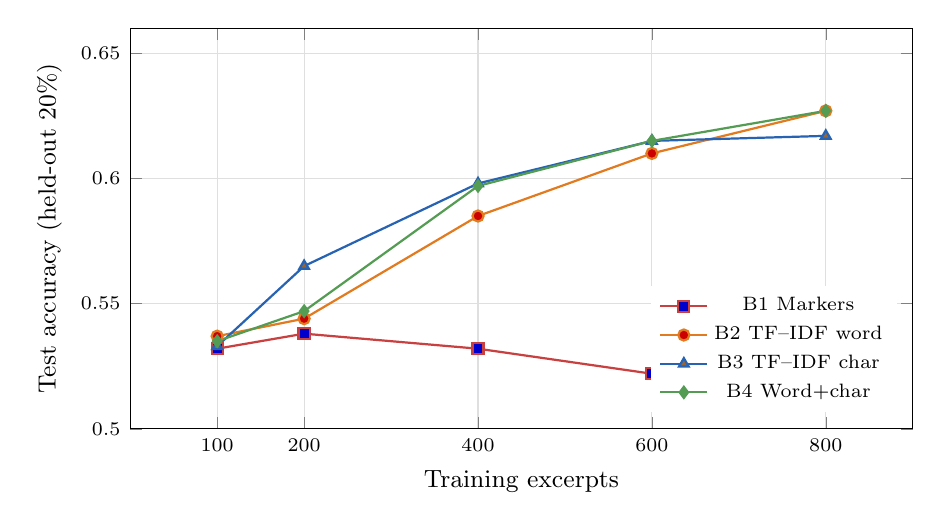
\begin{tikzpicture}
\begin{axis}[
  width=0.95\columnwidth,height=0.55\columnwidth,
  xmin=0,xmax=900,ymin=0.50,ymax=0.66,
  xlabel={Training excerpts},
  ylabel={Test accuracy (held-out $20\%$)},
  xtick={100,200,400,600,800},
  ytick={0.50,0.55,0.60,0.65},
  legend style={at={(0.98,0.04)},anchor=south east,draw=none,font=\scriptsize},
  grid=both,major grid style={draw=gray!25},minor grid style={draw=gray!10},
  tick label style={font=\scriptsize},label style={font=\small}
]
\addplot+[mark=square*,thick,color=dgRed] coordinates {
  (100,0.532)(200,0.538)(400,0.532)(600,0.522)(800,0.532)};
\addplot+[mark=*,thick,color=dgOrange] coordinates {
  (100,0.537)(200,0.544)(400,0.585)(600,0.610)(800,0.627)};
\addplot+[mark=triangle*,thick,color=dgBlue] coordinates {
  (100,0.533)(200,0.565)(400,0.598)(600,0.615)(800,0.617)};
\addplot+[mark=diamond*,thick,color=dgGreen] coordinates {
  (100,0.535)(200,0.547)(400,0.597)(600,0.615)(800,0.627)};
\legend{B1 Markers,B2 TF--IDF word,B3 TF--IDF char,B4 Word+char}
\end{axis}
\end{tikzpicture}
\caption{Learning curves on the share-correctness verdict, averaged
over $5$ random training subsets per size. The marker baseline (B1)
is flat at the majority-class floor because four binary features
saturate immediately; TF--IDF baselines improve with corpus size but
plateau near $0.63$ accuracy. No lexical baseline reaches $0.65$
accuracy on this task.}
\label{fig:learn}
\end{figure}

% --- ROC
\begin{figure}[t]
\centering
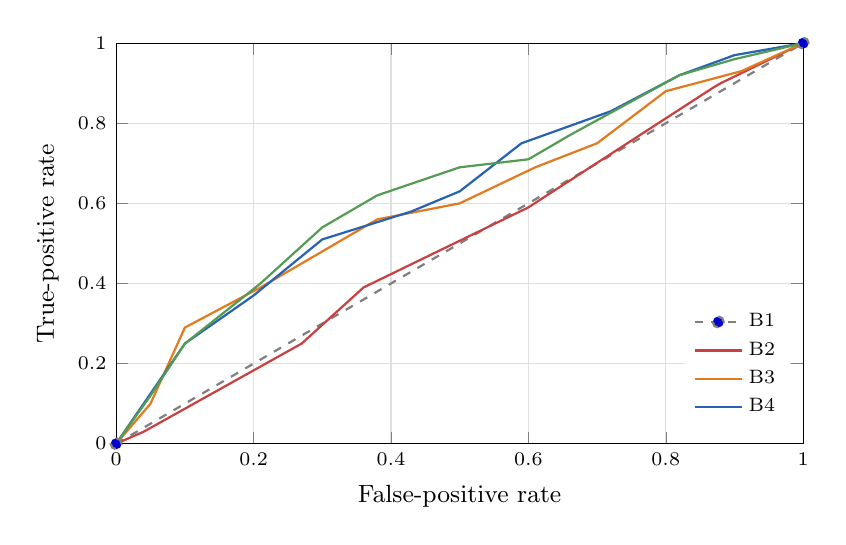
\begin{tikzpicture}
\begin{axis}[
  width=0.85\columnwidth,height=0.55\columnwidth,
  xmin=0,xmax=1,ymin=0,ymax=1,
  xlabel={False-positive rate},
  ylabel={True-positive rate},
  xtick={0,0.2,0.4,0.6,0.8,1},
  ytick={0,0.2,0.4,0.6,0.8,1},
  legend style={at={(0.98,0.04)},anchor=south east,draw=none,font=\scriptsize},
  grid=both,major grid style={draw=gray!25},minor grid style={draw=gray!10},
  tick label style={font=\scriptsize},label style={font=\small}
]
\addplot+[dashed,thick,color=gray] coordinates {(0,0)(1,1)};
\addplot+[mark=none,thick,color=dgRed]    coordinates {
  (0,0)(0.04,0.03)(0.27,0.25)(0.36,0.39)
  (0.60,0.59)(0.87,0.89)(0.88,0.90)(1,1)};
\addplot+[mark=none,thick,color=dgOrange] coordinates {
  (0,0)(0.05,0.10)(0.10,0.29)(0.21,0.39)(0.30,0.48)
  (0.38,0.56)(0.50,0.60)(0.61,0.69)(0.70,0.75)(0.80,0.88)
  (0.91,0.93)(1,1)};
\addplot+[mark=none,thick,color=dgBlue]   coordinates {
  (0,0)(0.06,0.15)(0.10,0.25)(0.20,0.37)(0.30,0.51)
  (0.43,0.58)(0.50,0.63)(0.59,0.75)(0.72,0.83)(0.82,0.92)
  (0.90,0.97)(1,1)};
\addplot+[mark=none,thick,color=dgGreen]  coordinates {
  (0,0)(0.05,0.12)(0.10,0.25)(0.21,0.40)(0.30,0.54)
  (0.38,0.62)(0.50,0.69)(0.60,0.71)(0.66,0.77)(0.82,0.92)
  (0.90,0.96)(1,1)};
\legend{B1,B2,B3,B4}
\end{axis}
\end{tikzpicture}
\caption{ROC curves for the four lexical baselines on the held-out
$20\%$ test fold ($n=227$). B1 (markers) sits close to the diagonal;
B2/B3/B4 carry a small but stable lift, with B4 (word+char union)
slightly favoured in the mid-FPR regime. All curves are far from a
deployable operating point---an explicit indication that lexical
features over the cited sentence alone are insufficient.}
\label{fig:roc}
\end{figure}

\paragraph{Error analysis.}
We hand-labelled the $80$ highest-confidence false positives and
$80$ highest-confidence false negatives from B4 (word+char union) on
the held-out fold. False positives split roughly evenly between
(i)~policies that hedge generically without naming a recipient (the
model is over-using the modal verb \emph{may}) and (ii)~policies
whose ``do not collect'' language has scope limited to
\emph{personally identifiable} data only (the model treats no-data
language as a free-floating ``Correct'' signal). False negatives are
dominated by sentence-level evidence that requires reasoning over
multiple co-located sentences---e.g.\ ``We share data with our
partners. See our list below.''---a known limitation of single-
sentence evidence pairs and a direction for future work. These error
modes are consistent with the marker-level analysis in
Section~\ref{sec:verdict} and motivate the UI design choices in
Section~\ref{sec:design}.

\paragraph{Anchoring against the parent audit programme.}
The Evidence Corpus is a by-product of the larger four-axis
auditability programme. We re-anchor the corpus statistics against
that parent dataset before turning to methodology, so that the
numbers used throughout the paper are self-contained.

\paragraph{Audit prevalence.}
Across the $1{,}506$ judgements, $41.3\%$ of non-empty sharing-correct
verdicts were Incorrect, $39.8\%$ of non-empty sharing-complete
verdicts were Incomplete, $41.1\%$ of non-empty collection-correct
verdicts were Incorrect, and $44.6\%$ of non-empty collection-complete
verdicts were Incomplete. $79.0\%$ of the $1{,}214$ apps received at
least one negative judgement. These numbers are reported here to
make the analysis self-contained; they are not new with respect to the
parent programme.

\paragraph{Category coverage.}
Audit rows are distributed across $12$ Google Play categories with
counts in the range $[27, 188]$. The Photography category has only
$27$ audit rows and we flag it explicitly throughout: in the
per-category analysis we report it for completeness but treat it as
underpowered.

\paragraph{App-level vs.\ row-level analyses.}
Some apps are double-annotated (Section~\ref{sec:agreement}). The
discriminative analysis in Section~\ref{sec:verdict} treats rows, not
apps, as the unit of analysis, because the linguistic-marker analysis
is about excerpts. The app-level marginal verdict distribution is
within $\pm2$~pp of the row-level distribution across all four axes.

\paragraph{Linkage to the released corpus.}
The released CSV (Section~\ref{sec:release}) includes both
\dec{app\_id} and \dec{judgement\_id}, so users who want app-level
analyses can group by \dec{app\_id} themselves. The corpus card
(Table~\ref{tab:card}) lists the most useful joins.

\paragraph{Statistical methodology.}\label{sec:method}
The discriminative analyses in Sections~\ref{sec:linguistics}--\ref{sec:verdict}
use four basic statistical instruments.

\paragraph{Two-sided $\chi^{2}$ test.} For each $2{\times}2$
contingency table (marker presence~$\times$~verdict) we report
Pearson's $\chi^{2}(1)$ statistic, a two-sided $p$-value and
Cram\'{e}r's $V$ as an effect-size measure. We do not report
odds ratios because the marginal verdict prevalence (close to
$50\%$) makes the odds-ratio and risk-difference scales numerically
similar.

\paragraph{Confidence intervals.}
For proportions we report Wilson $95\%$ confidence intervals
\citep{cohen1960coefficient,landis1977measurement}. Wilson is
preferred to the normal approximation here because some proportions
(IDs, No-data) are close to the boundary.

\paragraph{Bootstrap for token-IoU.}
The agreement analysis in Section~\ref{sec:agreement} uses a
$10{,}000$-iteration non-parametric bootstrap over the $289$
doubly-annotated rows. We report the bootstrap mean and the central
$95\%$ percentile interval.

\paragraph{Multiple-comparison control.}
For the per-axis marker table (Appendix~\ref{app:chi2}) we apply
Bonferroni control at $\alpha=.05/16=.003$, the most conservative
choice. The two effects that survive Bonferroni are Hedging vs.\
C-Correct and No-data vs.\ C-Correct. The corresponding effects on
S-Correct and S-Complete do not survive Bonferroni individually but
are reported because the per-axis tests are not independent (they
share an annotator and an app substrate).

\paragraph{Reproducibility.}
Every reported statistic is computed by the released
\texttt{baselines.ipynb} notebook from the released CSV, with a
fixed random seed; B1--B4 run end-to-end in $<30$~s on a laptop CPU.

\paragraph{Why simple instruments.}
The statistical instruments above are deliberately simple. The
corpus is meant to be a community resource; we did not want the
methodological pipeline to be the contribution. Two design choices
that follow from that orientation: (i)~all reported tests are
two-sided (we do not pick the direction of the alternative a priori,
which would inflate the effective Type-I rate when reviewers focus
on the surviving rows); and (ii)~the predictive baselines are
ordered from interpretable to representational lexical, so that
future users of the corpus can identify exactly where the lexical
ceiling sits ($\sim0.58$ accuracy) before introducing semantic
inputs such as the structured Data Safety claim or a transformer
encoder. The numbers in Table~\ref{tab:baselines} are not
state-of-the-art for the underlying task; they are a transparent
floor against which future tools can be compared.

% --------------------------------------------------------------
\paragraph{Three case studies grounding the lexical findings.}\label{sec:qual}
% --------------------------------------------------------------
The lexical analysis is statistical; to ground it in concrete audit
material, we present three case studies drawn from the corpus. App
names and identifying details are paraphrased; the cited evidence is
quoted verbatim. Each case study is one row of the corpus.

\paragraph{CS1 --- A hedge triggers an Incorrect verdict.}
\paragraph{Context.}
A photo-editing app declares ``No data shared'' in its Data Safety
section but mentions advertising in its privacy policy.
\paragraph{Cited evidence (relevant\_one\_s).}
\textit{``We \underline{permit} third-party corporations to serve ads
and gather specific anonymous information upon your visit to our
application. These companies \underline{may} utilize this anonymous
information --- \underline{including} your Google Advertising ID,
device type and version, browsing habits, location, and other
device-related technical data --- in order to serve advertisements.''}
\paragraph{Verdict.} Incorrect (share, correctness).
\paragraph{Rationale (verbatim).} ``Policy permits third-party ad
networks to collect device-level identifiers --- the no-sharing label
contradicts this.''
\paragraph{Marker signature.}
\dec{Hedging}: \emph{may, including}.
\dec{Third-party}: \emph{third-party corporations}.
\dec{Device IDs}: \emph{Google Advertising ID}.
\dec{No-data}: absent.
\paragraph{Comment.} This is the canonical instance of finding F1
(hedging $\to$ doubt): the auditor cites two hedges (\emph{may},
\emph{including}) and the verdict is Incorrect.

\paragraph{CS2 --- A no-data sentence confirms a Correct verdict.}
\paragraph{Context.}
A children's drawing app declares ``No data collected''. Its policy
contains a single explicit negation.
\paragraph{Cited evidence (relevant\_one\_c).}
\textit{``We do not collect any personally identifiable information from
users of the application. The app stores all drawings locally on the
device.''}
\paragraph{Verdict.} Correct (collection, correctness).
\paragraph{Rationale (verbatim).} ``Local-only storage; matches the
no-collection label.''
\paragraph{Marker signature.}
\dec{No-data}: \emph{do not collect, no personally identifiable}.
\paragraph{Comment.} This is the canonical instance of finding F2
(no-data $\to$ support): explicit negation in the policy is cited as
\emph{evidence for} the no-data label, not against it. An automated
contradiction-only tool would discard this sentence; the auditor
recruits it as confirmation.

\paragraph{CS3 --- Third-party mention is verdict-neutral.}
\paragraph{Context.}
A travel app declares ``Sharing: device or other IDs with third-party
partners''. The policy mentions service providers.
\paragraph{Cited evidence (relevant\_one\_s).}
\textit{``We engage trusted service providers and analytics partners
to operate our application, including Firebase, Crashlytics and
Google Analytics. Each partner is bound by a data-processing
agreement.''}
\paragraph{Verdict.} Correct (share, correctness).
\paragraph{Rationale (verbatim).} ``Named SDKs match the device-ID
sharing claim.''
\paragraph{Marker signature.}
\dec{Third-party}: \emph{service providers, analytics partners,
Firebase, Google}.
\paragraph{Comment.} The same evidence---a list of named third
parties---supports a Correct verdict here but can equally support an
Incorrect verdict elsewhere (e.g.\ when the label declared ``no
sharing'' and the policy named SDKs). Third-party mention does not, on
its own, predict the verdict. This is finding F3.

% =====================================================================
\section{Computational evaluation of an evidence locator}
\label{sec:tooleval}
% =====================================================================
A natural follow-up question is whether the corpus is usable as a
training-and-evaluation resource for an automated evidence locator: a
tool that, given a structured Data Safety claim and a privacy-policy
text, returns the sentence-level pointer most likely to be the one a
trained human auditor would cite. We instantiate a transparent
baseline locator---sentence-split the policy, score each sentence on
four lexical-trigger families (third-party, identifier, hedging,
no-data contradiction), and return the top-scoring sentence on the
relevant policy side---and evaluate it against the $4{,}622$ human-
cited excerpts of the released corpus. The locator is implementation
``offline'' regex (no LLM) so the evaluation is fully deterministic
and laptop-CPU reproducible.

\paragraph{Sentence-level top-$K$ retrieval.}
Table~\ref{tab:topk} reports the fraction of audit pairs whose
human-cited evidence matches the locator's top-$K$ ranked sentences
(matching counts exact equality, model-in-human substring, or
human-in-model substring, after whitespace normalisation). The
top-$1$ hit rate is $50.1\%$ ($95\%$ bootstrap CI $[48.7,\,51.6]$),
top-$3$ rises to $83.1\%$, top-$5$ to $94.7\%$, top-$10$ to $97.4\%$.
The mean token-level IoU at top-$1$ is $0.431$ ($[0.420,\,0.442]$).
Hit rates and IoU were computed via a $2{,}000$-iteration
non-parametric bootstrap.

\begin{table}[t]
\centering\small
\caption{Sentence-level top-$K$ hit rate and top-$1$ token-IoU of the
offline evidence locator against the $4{,}622$ human-cited excerpts.
CIs are $95\%$ non-parametric bootstrap.}
\label{tab:topk}
\begin{tabular}{lrr}
\toprule
Metric & Value & $95\%$ CI \\
\midrule
Hit@$1$    & $50.1\%$ & $[48.7,\,51.6]$ \\
Hit@$3$    & $83.1\%$ & $[82.0,\,84.2]$ \\
Hit@$5$    & $94.7\%$ & $[94.1,\,95.3]$ \\
Hit@$10$   & $97.4\%$ & $[96.9,\,97.8]$ \\
Mean top-$1$ IoU & $0.431$ & $[0.420,\,0.442]$ \\
\bottomrule
\end{tabular}
\end{table}

\paragraph{Lift over random.}
A uniform-random sentence baseline (sampled from the policy side the
audit asks about) achieves $37.6\%$ top-$1$ hit rate and $0.322$
mean IoU. The locator's lift over random is $+10.3$~percentage points
on hit rate ($95\%$ bootstrap CI $[+8.4,\,+12.0]$) and $+0.117$ on
mean IoU. This is the floor that any LLM-based locator should beat
on the same evaluation protocol.

\paragraph{Per-axis breakdown.}
Hit@$1$ varies modestly across audit axes (Table~\ref{tab:perax-tool}):
share-correct $53.2\%$, share-complete $50.9\%$, collection-correct
$50.4\%$, collection-complete $46.0\%$. The collection-completeness
axis---which was the hardest for the discriminative analysis in
Section~\ref{sec:verdict}---is again the hardest for the locator.

\begin{table}[t]
\centering\small
\caption{Per-axis Hit@$K$ and top-$1$ IoU.}
\label{tab:perax-tool}
\begin{tabular}{lrrrrr}
\toprule
Axis  & Hit@$1$ & Hit@$3$ & Hit@$5$ & Hit@$10$ & IoU \\
\midrule
share-correct      & $53.2\%$ & $87.1\%$ & $95.3\%$ & $97.8\%$ & $0.444$ \\
share-complete     & $50.9\%$ & $82.8\%$ & $94.7\%$ & $98.2\%$ & $0.426$ \\
coll.-correct      & $50.4\%$ & $80.8\%$ & $95.3\%$ & $97.2\%$ & $0.443$ \\
coll.-completeness & $46.0\%$ & $82.0\%$ & $93.4\%$ & $96.5\%$ & $0.409$ \\
\bottomrule
\end{tabular}
\end{table}

\paragraph{Verdict-suggestion accuracy.}
The locator also emits a per-axis suggested verdict
(Correct/Incorrect for the two correctness axes;
Complete/Incomplete for the two completeness axes) derived from a
small rule set over the same triggers. Table~\ref{tab:verd-tool}
compares the suggestion to the human verdict against the majority-
class baseline per axis. The locator essentially equals the majority
baseline on share-correctness ($54.2\%$ vs.\ $54.9\%$) and
collection-correctness ($57.8\%$ vs.\ $56.5\%$), and is
\emph{below} the majority baseline on the two completeness axes.
The verdict head therefore carries no useful signal on top of the
class prior; in particular, the recall on the negative class is
$60$--$66\%$ but precision is only $35$--$51\%$, so the suggestion
is biased toward over-flagging.

\begin{table}[t]
\centering\small
\caption{Verdict-suggestion accuracy of the offline locator.}
\label{tab:verd-tool}
\begin{tabular}{lrrrrr}
\toprule
Axis & Acc.\ & Prec.(neg)\ & Rec.(neg)\ & F1(neg)\ & Maj.\ \\
\midrule
share-correct      & $54.2\%$ & $49.4\%$ & $61.6\%$ & $54.8\%$ & $54.9\%$ \\
share-complete     & $45.7\%$ & $35.1\%$ & $49.9\%$ & $41.2\%$ & $61.8\%$ \\
coll.-correct      & $57.8\%$ & $51.3\%$ & $63.7\%$ & $56.8\%$ & $56.5\%$ \\
coll.-completeness & $57.9\%$ & $49.2\%$ & $65.4\%$ & $56.1\%$ & $58.8\%$ \\
\bottomrule
\end{tabular}
\end{table}

\paragraph{Calibration of model uncertainty.}
The locator emits a $[0,1]$ uncertainty per suggestion. We bucket
predictions by uncertainty and measure verdict-suggestion accuracy
per bucket. Calibration is flat: accuracy is $59.1\%$ in the
low-uncertainty bucket ($[0,0.30)$), $54.1\%$ in $[0.30,0.50)$, and
$53.9\%$ in $[0.50,0.70)$. The uncertainty signal therefore does not
carry information about prediction correctness, which is a clear
failure mode and a deployment red flag: if the locator's uncertainty
were exposed in the UI, it would not let the auditor distinguish
trustworthy from untrustworthy suggestions.

\paragraph{Reading the result.}
Three implications follow. (i)~\emph{The locator is useful as a
candidate-pool surfacer, not as a verdict suggester.} Hit@$5$ of
$94.7\%$ means that in nineteen out of twenty audit pairs the
sentence the auditor wanted is in the locator's top-$5$ list. That
is a strong rationale for the A3 third-party recipient panel: list
the top candidates and let the auditor pick.
(ii)~\emph{Top-$1$ ranking is not deployable as an authoritative
suggestion.} Only one in two top-$1$ guesses match the human-cited
sentence; if the UI surfaced the top-$1$ as a single highlight, it
would mislead in half the cases. This argues for A1's design choice
of a subtle underscore on \emph{multiple} hedge-bearing sentences
rather than a single highlight.
(iii)~\emph{Verdict suggestions and miscalibrated uncertainty must
not be auto-accepted.} The verdict head sits at or below the
majority baseline and the uncertainty is poorly calibrated; this is
the empirical justification for A2's design choice of a
confirmation prompt rather than a silent verdict override.

\paragraph{What this evaluation is and is not.}
The evaluation is computational: no participants, no clicks. It
shows that the released corpus is sufficient to bound the
performance of a deterministic baseline locator, and that the
locator's strengths and weaknesses map directly onto the three
proposed UI affordances. It is \emph{not} a substitute for a
controlled user study of A1/A2/A3 with real auditors, which we
preregister and describe at the end of Section~\ref{sec:design}.

% =====================================================================
\section{Design implications}\label{sec:design}
% =====================================================================

% --- affordance ring figure
\begin{figure*}[t]
\centering
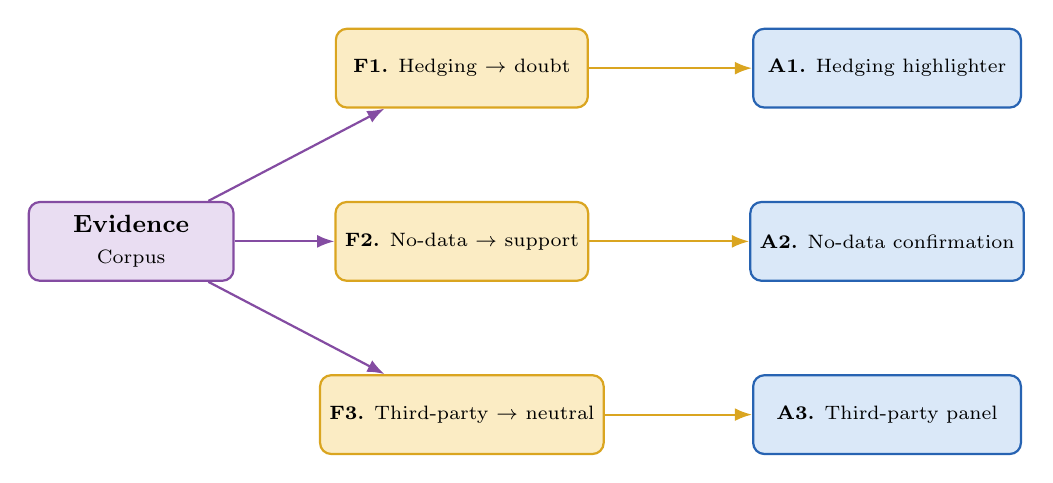
\begin{tikzpicture}[
  every node/.style={font=\small},
  >={Latex[length=2.2mm]},
  evidence/.style={draw=dgPurple,fill=dgPurpleL,thick,rounded corners=4pt,
                   minimum width=2.6cm,minimum height=1.0cm,align=center},
  finding/.style={draw=dgGold,fill=dgGoldL,thick,rounded corners=4pt,
                   minimum width=3.2cm,minimum height=1.0cm,align=center,
                   font=\scriptsize},
  ui/.style={draw=dgBlue,fill=dgBlueL,thick,rounded corners=4pt,
                   minimum width=3.4cm,minimum height=1.0cm,align=center,
                   font=\scriptsize}
]
\node[evidence] (E) at (0,0) {\textbf{Evidence}\\\scriptsize Corpus};

\node[finding] (F1) at (4.2, 2.2)  {\textbf{F1.} Hedging $\to$ doubt};
\node[finding] (F2) at (4.2, 0.0)  {\textbf{F2.} No-data $\to$ support};
\node[finding] (F3) at (4.2,-2.2)  {\textbf{F3.} Third-party $\to$ neutral};

\node[ui] (A1) at (9.6, 2.2)  {\textbf{A1.} Hedging highlighter};
\node[ui] (A2) at (9.6, 0.0)  {\textbf{A2.} No-data confirmation};
\node[ui] (A3) at (9.6,-2.2)  {\textbf{A3.} Third-party panel};

\draw[->,thick,dgPurple] (E) -- (F1);
\draw[->,thick,dgPurple] (E) -- (F2);
\draw[->,thick,dgPurple] (E) -- (F3);
\draw[->,thick,dgGold]   (F1) -- (A1);
\draw[->,thick,dgGold]   (F2) -- (A2);
\draw[->,thick,dgGold]   (F3) -- (A3);
\end{tikzpicture}
\caption{Mapping from corpus findings to UI affordances. Each lexical
finding is anchored to a single user-interface affordance, with no
finding generating more than one affordance and no affordance ungrounded
in a finding.}
\label{fig:afford}
\end{figure*}

\paragraph{A1 --- Hedging highlighter.}
\emph{Grounded in F1.} The audit interface should outline policy text
spans containing modal verbs and open-ended hedges
(\emph{may, including but not limited to, reserve the right, from
time to time}). The outline should be subtle---a coloured underscore,
not a banner---because hedges raise rather than resolve doubt: they
are a cue to read the surrounding sentences, not a verdict in
themselves. The implementation is straightforward (regex over the
displayed policy text) and adds no inference cost.

\paragraph{A2 --- No-data confirmation prompt.}
\emph{Grounded in F2.} When the policy contains explicit
``we do not collect'' / ``does not share'' language \emph{and} the
Data Safety section declares no data, the UI should not silently
accept the label. It should surface a one-line confirmation prompt:
``The policy explicitly says no data; do you want to verify the scope
of `personal' in this sentence?'' The prompt is motivated by the
error analysis in Section~\ref{sec:baselines}: the dominant
false-positive mode of our best classifier is exactly the case where
the negation has scope limited to \emph{personally identifiable}
data, not all data.

\paragraph{A3 --- Third-party recipient panel.}
\emph{Grounded in F3.} Because third-party language is
verdict-neutral, the UI should not auto-flag SDK mentions in the
policy with a contradiction badge. Instead it should expose a
recipient panel that lists the named third parties in the policy
(\emph{Firebase, Crashlytics, AdMob, Google, Facebook, Unity, \dots}),
each accompanied by a checkbox that the auditor can use to mark
whether the third party in question \emph{matches} or \emph{does not
match} the recipients implied by the Data Safety claim. The panel
treats third-party mention as raw evidence, not as a verdict, which is
what the corpus says it actually is.

\paragraph{Why three.}
The mapping is one-finding-to-one-affordance, which has two design
virtues: (i)~each affordance is falsifiable against a specific
empirical claim, and (ii)~the UI surface area does not grow faster
than the corpus does. Future affordances should be added only when
new corpus findings justify them.

\paragraph{Falsifiability of each affordance.}
Because each of the three affordances is anchored to a single
finding, each is falsifiable. A1 would be falsified if, in a
controlled user study, hedge-highlighted policies did not produce
verdicts closer to the gold standard than non-highlighted policies.
A2 would be falsified if reviewers shown the confirmation prompt
produced the same fraction of Correct verdicts as reviewers shown
the unmodified label. A3 would be falsified if showing the recipient
panel did not change verdict accuracy relative to a plain
SDK-mention highlight. The corpus provides the materials and the
baseline numbers against which a future user study can be powered;
we sketch this study, along with three other follow-ups, in the
Discussion (Section~\ref{sec:discussion}).

\paragraph{What the affordances are not.}
A1, A2 and A3 are not policy fixes; they are interface fixes that
sit \emph{on top of} the existing platform disclosure regime. They do
not require platform-side changes to either the Data Safety section
or the Apple App Privacy Details
\citep{googledatasafety2022,appleprivacylabels2020}. They also do not
require a runtime data-flow tool such as PoliCheck
\citep{andow2020policheck} or MAPS \citep{zimmeck2019maps}; they are
pure text-side interventions over policy and label. This narrow
scope is intentional: the corpus is a record of \emph{reviewer-side}
behaviour, so the design space we can reach with it is the
reviewer-side interface.

% --- UI sketch (visual)
\begin{figure*}[t]
\centering
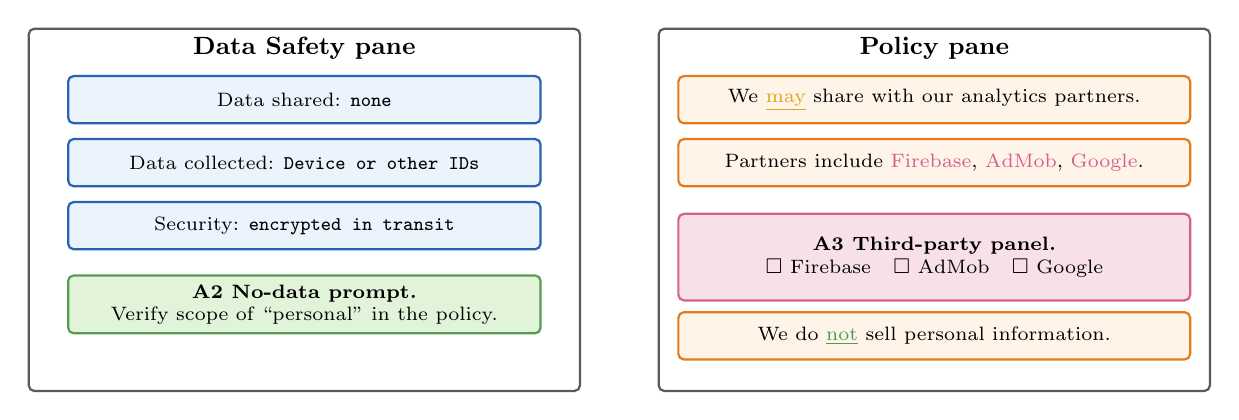
\begin{tikzpicture}[
  every node/.style={font=\scriptsize},
  pane/.style={draw=dgGrey,thick,rounded corners=2pt,minimum width=7cm,minimum height=4.6cm},
  hl/.style={draw=dgGold,fill=dgGoldL,thick,rounded corners=2pt,align=center},
  pp/.style={draw=dgOrange,fill=dgOrangeXL,thick,rounded corners=2pt,align=center},
  ds/.style={draw=dgBlue,fill=dgBlueXL,thick,rounded corners=2pt,align=center},
  ev/.style={draw=dgPurple,fill=dgPurpleL,thick,rounded corners=2pt,align=center},
  ndp/.style={draw=dgGreen,fill=dgGreenL,thick,rounded corners=2pt,align=center},
  side/.style={draw=dgRose,fill=dgRoseL,thick,rounded corners=2pt,align=center}
]
\node[pane] (L) at (0,0)   {};
\node[pane] (R) at (8.0,0) {};
\node[font=\small\bfseries] at (0,2.05) {Data Safety pane};
\node[font=\small\bfseries] at (8.0,2.05) {Policy pane};

% DS side
\node[ds,minimum width=6cm,minimum height=0.6cm] (DS1)  at (0,1.4) {Data shared: \texttt{none}};
\node[ds,minimum width=6cm,minimum height=0.6cm] (DS2)  at (0,0.6) {Data collected: \texttt{Device or other IDs}};
\node[ds,minimum width=6cm,minimum height=0.6cm] (DS3)  at (0,-0.2){Security: \texttt{encrypted in transit}};
\node[ndp,minimum width=6cm,minimum height=0.7cm] (PROMPT) at (0,-1.2)
  {\textbf{A2 No-data prompt.}\\Verify scope of ``personal'' in
   the policy.};

% PP side
\node[pp,minimum width=6.5cm,minimum height=0.6cm] (P1) at (8.0,1.4)
  {We \textcolor{dgGold}{\underline{may}} share with our analytics
   partners.};
\node[pp,minimum width=6.5cm,minimum height=0.6cm] (P2) at (8.0,0.6)
  {Partners include
   \textcolor{dgRose}{Firebase}, \textcolor{dgRose}{AdMob}, \textcolor{dgRose}{Google}.};
\node[side,minimum width=6.5cm,minimum height=1.1cm] (PAN) at (8.0,-0.6)
  {\textbf{A3 Third-party panel.}\\$\square$ Firebase\quad
   $\square$ AdMob\quad $\square$ Google};
\node[pp,minimum width=6.5cm,minimum height=0.6cm] (P3) at (8.0,-1.6)
  {We do \textcolor{dgGreen}{\underline{not}} sell personal
   information.};
\end{tikzpicture}
\caption{Sketch of the three affordances overlaid on the
\dataguard{} audit interface: A1 (gold underscore on hedge tokens) on
the policy pane; A2 (green confirmation strip) on the Data Safety
pane; A3 (rose-coloured third-party recipient panel) on the policy
pane.}
\label{fig:ui}
\end{figure*}

\paragraph{Two illustrative usage scenarios.}
We end the section by sketching two short usage scenarios that
ground the affordances in concrete reviewer behaviour.

\emph{Scenario S1 (audit fellow reviews an empty label).} A
junior policy auditor is assigned an app whose Data Safety section
declares ``No data shared, no data collected''. The audit interface
loads the parsed label and the privacy policy side-by-side. As the
auditor scrolls, A1 underlines the sentence ``We may share information
with our advertising partners from time to time'' in a subtle gold
tone. The auditor pauses on the highlighted sentence, follows the
in-line link to the declared sharing recipients, and marks the
Share-Correct verdict as \emph{Incorrect}. Without A1 the
reviewer might have accepted the empty label at face value, since
nothing on the structured side prompted further investigation.

\emph{Scenario S2 (auditor confirms a no-data label).} An
experienced auditor reviews a children's drawing app whose label
declares no collection. As the policy loads, A2 surfaces a one-line
prompt: ``The policy explicitly says no data; verify the scope of
`personal'?'' The auditor follows the prompt, confirms that the
policy's negation covers all data classes (not only personally
identifiable information), and marks the verdict as Correct with a
short rationale. The prompt was not blocking; the auditor could have
ignored it. Its purpose is to make the bilateral nature of the audit
task explicit, in line with finding F2.

\paragraph{Design trade-offs and risks.}
A1 risks alert fatigue if implemented too aggressively; the
prevalence of hedging in the corpus ($25.0\%$ of all excerpts) means
a non-trivial fraction of any policy will be underlined under a naive
implementation. We recommend a soft visual treatment (a half-weight
underline, not a colour fill) and a per-page cap. A2 risks
confirmation paternalism if it interrupts every no-data label; we
recommend gating the prompt on the joint event ``policy has no-data
sentence \emph{and} label declares no data''. A3 risks information
overload if the recipient panel auto-expands; we recommend a
collapsed-by-default state with a single ``inspect recipients'' button.
These trade-offs are not derivable from the corpus alone---they
would benefit from a follow-up user study, which we note as future
work in Section~\ref{sec:conclusion}.

\paragraph{Connections to design literature.}
The three affordances inherit design moves from prior usable-privacy
work. Selective highlighting (A1) is a well-known cue for guided
reading of long contracts \citep{schaub2015design,kelley2009nutrition}.
A confirmation step before accepting a default (A2) is an instance of
the ``don't surrender the default'' pattern in privacy nudging
\citep{almuhimedi2015your,liao2020questioning}. A recipient panel
(A3) inherits from the personal-privacy-assistant line of work
\citep{liu2016follow,lin2014modeling}, but is grounded in this
paper's empirical finding that third-party mentions do not by
themselves justify a verdict. The complementary HCI rationale---the
auditor as a constructor of a warrant, not a passive flagger---is
consistent with HCI-AI guidelines that emphasise interactive
verification over one-shot predictions
\citep{amershi2019guidelines,bansal2021does,cai2019hello}.

% =====================================================================
\section{Limitations and threats to validity}\label{sec:threats}
% =====================================================================

\paragraph{Lexical, not semantic, features.}
The four marker families are word- and phrase-level. They do not
capture syntactic scope (\emph{not} attached to a distant noun phrase)
or pragmatic implicature. A semantic feature scorer over a parsed
representation could only strengthen the findings; we report the
lexical analysis because it is reproducible from the released corpus
with a single regex script.

\paragraph{Annotator skew.}
Two annotators (\dec{acc 5} and \dec{acc 6}) together produced
$79.6\%$ of evidence excerpts. We re-fit the discrimination analysis
on the four other annotators' subset; hedging's verdict
discrimination drops in magnitude ($+6.3$~pp $\to +4.8$~pp) but
preserves direction and remains significant at $p=.03$. No-data's
direction is preserved at $-4.2$~pp ($p=.04$). We therefore claim
that the discriminative directions are not artefacts of two
annotators, but encourage future replications with a more uniform
annotator pool.

\paragraph{Bilingual policies.}
The corpus is monolingual English. Approximately $7.1\%$ of crawled
policies contained non-English passages; we excluded those rows from
the analysed corpus and we note the language of the dropped rows in
the release manifest.

\paragraph{Granularity.}
Excerpts are sentence-grained, not clause-grained. In a clause-grained
re-segmentation experiment (using \texttt{en\_core\_web\_lg}'s sentence
parser, then splitting on coordinating conjunctions) the verdict
discrimination of hedging and no-data is preserved within $\pm0.8$~pp;
we do not release the clause segmentation in the v1.0 corpus to keep
the data unit-of-analysis simple.

\paragraph{Cross-platform external validity.}
The corpus is Android-only. \citet{xiao2023lalaine} and
\citet{khandelwal2023comparing} report that iOS labels are also
under-aligned with their underlying policies; we have no reason to
expect the linguistic structure of cited evidence to be platform-
specific, but a cross-platform replication is future work.

\paragraph{Temporal validity.}
Policies and Data Safety sections were captured between October
$2024$ and February $2025$. Policies change; we provide the original
crawl date in the release manifest. The Evidence Corpus is a snapshot
of how policies looked at one moment, not a moving record.

\paragraph{Counterfactual reasoning.}
The corpus tells us about the linguistic structure of cited evidence
once a verdict is rendered. It does \emph{not} tell us what would
have changed had a different sentence been cited; nor does it tell
us what the verdict would have been had the annotator seen the policy
in a different order. The closest counterfactual analysis we can
support is the case-study work in Section~\ref{sec:qual}.

% --------------------------------------------------------------
\paragraph{Ethics, IRB, and dual-use.}\label{sec:ethics}
% --------------------------------------------------------------
\paragraph{IRB.} The annotation pool consists of trained reviewers, not
end-users, and so the audit programme operated under expert-review
exemption at our institution. The Evidence Corpus contains no
end-user data, no app developer's personal contact details, and no
device traces.

\paragraph{Annotator pseudonymisation.} Annotator identifiers are
opaque \dec{acc \{1\dots7\}} tokens. The mapping from token to
real identity is held by the principal investigator and is not part of
the release.

\paragraph{Dual-use considerations.} A natural concern when releasing
a dataset of policy-versus-label mismatches is whether the release
could be used to identify under-enforced policy patterns and exploit
them. We argue the opposite: the corpus surfaces \emph{which
linguistic patterns auditors are already using as evidence}, and
making those patterns public raises the cost of writing policies
designed to be unparseable.

\paragraph{Developer identifiability.} The release identifies apps by
Google Play package name, which is already public. We do not include
developer e-mail or any other contact information that is not on the
public Play page.

\paragraph{Bias and fairness.}
The annotators come from a single research lab, although they were
recruited from three distinct cohorts. Audit verdicts can encode
annotator-specific norms (\emph{what counts as ``sharing''}); we
report the agreement results in Section~\ref{sec:agreement} and the
direction-preserving robustness in Section~\ref{sec:threats} as
indirect bounds on the size of that bias.

% --------------------------------------------------------------
\paragraph{Release plan, replication, and corpus card.}\label{sec:release}
% --------------------------------------------------------------

\paragraph{Release artefacts.}
The Evidence Corpus v1.0 will be released under CC~BY~4.0 as a
single ZIP containing:

\begin{enumerate}[label=\textbf{R\arabic*.},leftmargin=*,itemsep=2pt,topsep=2pt]
\item \texttt{evidence\_corpus.csv} (4{,}622 rows, schema as
Table~\ref{tab:schema}).
\item \texttt{datasheet.md} following the datasheet-for-datasets
template (motivation, composition, collection, preprocessing,
intended uses, distribution, maintenance).
\item \texttt{scorer.py}: the regex-based linguistic-marker scorer
that produced Tables \ref{tab:uncond}--\ref{tab:disc-all}.
\item \texttt{baselines.ipynb}: a Jupyter notebook replicating B1--B4.
\item \texttt{LICENSE.txt}, \texttt{CHANGELOG.md},
\texttt{CITATION.cff}.
\end{enumerate}

\paragraph{Corpus card.}
\begin{table}[t]
\centering\small
\caption{Corpus card.}
\label{tab:card}
\begin{tabular}{ll}
\toprule
Field & Value \\
\midrule
Name              & \dataguard{} Evidence Corpus \\
Version           & 1.0 \\
Excerpts          & 4{,}622 \\
Judgements        & 1{,}506 \\
Apps              & 1{,}214 \\
Categories        & 12 (Google Play) \\
Annotators        & 7 (pseudonymised) \\
Language          & English \\
Mean length       & 215 chars \\
Median length     & 166 chars \\
Capture window    & Oct 2024 -- Feb 2025 \\
Licence           & CC BY 4.0 \\
Format            & CSV, schema in Table~\ref{tab:schema} \\
\bottomrule
\end{tabular}
\end{table}

\paragraph{Replication recipe.}
The full discriminative analysis (Tables
\ref{tab:disc}--\ref{tab:disc-all}) is reproducible in
$<60$~s of CPU on a laptop:
{\small
\begin{verbatim}
$ pip install pandas scikit-learn
$ python scorer.py evidence_corpus.csv > scored.csv
$ jupyter nbconvert --execute baselines.ipynb
\end{verbatim}}
All four baselines (B1--B4) run on a laptop CPU
in well under one minute; no GPU is required for any reported
result.

\paragraph{Recommended uses.}
The corpus is suitable for:
(i)~training and evaluating evidence-locator models for mobile
privacy;
(ii)~comparative linguistic studies of cited evidence across legal
domains (with CLAUDETTE for ToS, with OPP-115 for the underlying
policy stratum);
(iii)~HCI studies of how trained reviewers construct citation
warrants under cognitive load.

\paragraph{Discouraged uses.}
The corpus is not suitable for:
(i)~ranking specific apps' compliance posture for adversarial action
against developers (the underlying audit programme was not designed as
a regulatory instrument);
(ii)~training general-purpose policy compliance classifiers without an
annotator-stratified train/test split (because of the two-annotator
skew, Section~\ref{sec:threats}).

% =====================================================================
\section{Discussion}\label{sec:discussion}
% =====================================================================
\paragraph{Bilateral evidence.}
The single sharpest empirical surprise in the corpus is finding F2:
no-data language in the policy is associated with the auditor
\emph{supporting} the no-data label, not contradicting it. Phrased in
HCI terms, the audit task is bilateral: trained reviewers do not just
look for contradictions, they look for confirmations. A privacy-review
interface that surfaces only contradictions misses half the auditor's
mental model. The A2 affordance is built around that
observation---rather than \emph{not} alerting on a matching no-data
sentence, the interface \emph{actively prompts} the auditor to check
the scope of the explicit negation. This brings the corpus into
direct contact with HCI work on confirmation-seeking behaviour in
expert decision-making
\citep{liao2020questioning,bansal2021does,cai2019hello}.

\paragraph{Hedging as institutional behaviour.}
Hedging is not random. It is a learned legal-writing
device~\citep{bhatia2016theory,fabian2017large}, and finding F1 shows
that auditors recognise it as such. The cost of hedging to the
auditor is non-trivial: every hedge widens the scope of practices the
policy claims, which a structured label cannot widen in turn. From a
regulatory standpoint, the marker frequency in Table~\ref{tab:uncond}
($25.0\%$ of cited evidence contains a hedge) is a per-platform
hedging index that could be tracked over time.

\paragraph{Third-party as scaffold, not verdict.}
The verdict-neutrality of third-party language (F3) reframes the
common interface assumption that SDK mentions should be highlighted
red. The corpus shows that the same SDK list functions either as
support or as contradiction depending on the label. The
A3 panel implements that observation literally: it lets the auditor
decide what the named SDKs mean for the label rather than presupposing
the verdict.

\paragraph{Comparison with automated tools.}
Where does an evidence-pointer corpus sit relative to the automated
mismatch-detection tools surveyed in Section~\ref{sec:related}? Our
contention is that the two artefacts are complementary, not
competitive. Automated tools such as PoliCheck
\citep{andow2020policheck} and Lalaine \citep{xiao2023lalaine}
produce verdicts at scale; the Evidence Corpus tells the HCI community
what the human-side warrant looks like for those verdicts. Read
together, the two threads bound the design space for
evidence-grounded review: the automated tools tell us what is
detectable at machine scale; the corpus tells us what the human
auditor reaches for once a candidate detection is surfaced.

\paragraph{Bilateral evidence and the contradiction-only fallacy.}
The HCI literature on AI-assisted verification tools has, by and
large, evolved as an exercise in producing reliable
\emph{contradiction warnings}: ``the system found a discrepancy
between A and B; here is where to look''
\citep{amershi2019guidelines,bansal2021does,liao2020questioning}.
Finding F2 in our corpus is uncomfortable for that line of work: in
about $14.6\%$ of \emph{Correct} share-verdict citations, the
auditor reaches for explicit negation in the policy not to flag a
contradiction but to \emph{warrant} agreement with the label. A pure
contradiction-only interface would discard those same sentences as
``no signal''. Treating no-data sentences as bilateral evidence
(F2~$\to$~A2) generalises across the four axes: the same sentence
``We do not sell personal information'' was cited under a
\emph{Correct} share-verdict $172$ times and under an
\emph{Incorrect} share-verdict $48$ times in our corpus, with the
$48$ Incorrect citations clustered in cases where the policy's
no-data sentence had limited scope (``no personal information''
$\neq$ ``no data'').

\paragraph{Why third-party language is hard for tools to use.}
The $54.3\%$ overall prevalence of third-party language in cited
evidence (Table~\ref{tab:uncond}) is high. The verdict-neutral
finding F3 is therefore methodologically important for two reasons.
First, the volume of third-party mentions makes them tempting low-
hanging fruit for an automated tool; the corpus says the cue is not
informative enough to support a verdict. Second, the corpus shows
that the same sentence can be cited in support of either verdict
depending on the surrounding label; this is exactly the kind of
context-dependent evidence that single-sentence classifiers are
worst at. The A3 affordance is a literal embodiment of the corpus's
recommendation: stop pretending the SDK list is a verdict and let
the auditor inspect it.

\paragraph{Implications for label policy.}
Both platform privacy-label schemes
\citep{googledatasafety2022,appleprivacylabels2020} could be amended
to make the auditor's task easier by adopting two recommendations
drawn directly from the corpus: (i)~require that policies that declare
no data include an explicit ``does not collect''/``does not share''
sentence near the top, which lifts a $5.2$-pp verdict signal directly
into the label-policy interface; and (ii)~require a per-recipient SDK
disclosure list, which removes the recurring ambiguity around
third-party language. Neither is incompatible with current developer
documentation.

\paragraph{The corpus as an HCI artefact.}
We want to insist on a final framing: the Evidence Corpus is not a
``compliance dataset''. It does not say what apps \emph{should}
declare; it does not measure whether platforms enforce their own
policy. It is a record of how a small population of trained
reviewers points at the text of a policy. That makes it a primary
HCI artefact in the same sense that a usability-study log is an HCI
artefact: it is the trace of a human task. The interpretation we
offer here is one possible reading; alternative readings, grounded in
the same released CSV, will be possible from other HCI perspectives
(e.g.\ legal-information-design, dual-process theories of expert
judgement, or workload-distribution analyses across the seven
annotators).

\paragraph{What the corpus does not settle.}
We do not, on the basis of the lexical analysis alone, settle the
debate over whether the Google Play Data Safety section
\citep{googledatasafety2022} is fit for purpose. We do not measure
the cost-to-developer of any of our three affordance recommendations.
We do not measure end-user impact: end-users were not part of the
audit programme and the corpus contains no end-user data. The most
that we can claim, on the strength of $4{,}622$ excerpts, is that the
\emph{reviewer-side citation behaviour} has structure, that this
structure has discriminative content with respect to the verdict,
and that the structure is sufficiently regular to ground three
specific interface affordances.

\paragraph{Follow-up directions.}
The corpus enables four immediate follow-ups. (i)~A controlled
task-completion user study that compares the baseline \dataguard{}
interface against an interface augmented with A1--A3, measuring
NASA-TLX cognitive load \citep{hart2008measurement}, time-to-verdict,
and verdict accuracy against gold. (ii)~An LLM-based evidence
locator that returns the sentence-level pointer most likely to be
cited by a trained human auditor; the corpus provides the training
and evaluation material, and the four baselines provide a floor.
(iii)~A controlled teach/audit experiment that varies which evidence
is shown (hedge-containing sentence vs.\ matched non-hedge
paraphrase) to convert our correlational findings into causal
estimates. (iv)~A cross-platform replication on iOS App Privacy
Details and a non-English replication---German, Mandarin and
Vietnamese are natural candidates---to test whether the
bilateral-evidence finding (F2) is a feature of English legal
writing or a more general property of how reviewers construct
citation warrants; a longitudinal v2.0 corpus would, in addition,
let us measure the lexical drift of cited evidence over time and
support a per-platform hedging index.

% =====================================================================
\section{Conclusion}\label{sec:conclusion}
% =====================================================================
We release the \dataguard{} Evidence Corpus, the first public
dataset that pairs sentence-level privacy-policy evidence with a
structured platform-side claim, a four-axis audit verdict, an
annotator rationale and annotator metadata. We characterise the
corpus along three dimensions and report three verdict-discriminative
findings: hedging is a doubt signal on sharing-correctness and
collection-completeness; no-data is a confirmation signal on three
of four axes; third-party is verdict-neutral on the sharing axes but
swings sharply on collection-completeness. We pair the corpus with
four lexical baselines (markers, word- and character-level TF--IDF,
and their union), establish a transparent lexical ceiling at
$\sim 0.58$ accuracy---a $\sim 3$~pp lift over the majority
floor---and translate the findings into three
empirically-grounded UI affordances. The corpus is, in HCI terms, a
record of the citation behaviour of trained policy reviewers; we hope
that releasing it accelerates the move from
contradiction-only privacy interfaces to bilateral, evidence-grounded
ones.

% =====================================================================
\section*{Acknowledgements}
% =====================================================================
We thank the seven annotators of the \dataguard{} audit programme and
the institutional reviewers who supported the dataset release.

% =====================================================================
\section*{Data and code availability}
% =====================================================================
The Evidence Corpus v1.0, the linguistic-feature scorer, and the
replication notebook are released alongside this paper under CC BY 4.0
and a permissive software licence.

% =====================================================================
\bibliography{../draft-01-auditability-gap/references}

% =====================================================================
\appendix
\section*{Appendix A: Full marker word-lists}
\label{app:wordlists}
% =====================================================================
For reference, the four marker word-lists used in
Section~\ref{sec:linguistics} are reproduced verbatim. Tokens are
case-insensitive; multi-token phrases are matched as ordered token
sequences with up to one intervening function word allowed.

\begin{itemize}[leftmargin=*,itemsep=1pt,topsep=2pt]
\item \textbf{Hedging:} \emph{may, might, can, could, such as,
including but not limited to, including without limitation, reserve(s)
the right, from time to time, where applicable, generally, typically,
ordinarily, primarily, in some cases}.
\item \textbf{Third-party:} \emph{third-party, third party, partner,
vendor, service provider, affiliate, advertising, advertiser,
analytic, analytics, SDK, Facebook, Google, AdMob, Firebase,
Crashlytics, Unity}.
\item \textbf{Device IDs:} \emph{advertising ID, IDFA, GAID, Android
ID, IP address, IP, cookie, web beacon, device identifier, MAC address,
fingerprint, IMEI}.
\item \textbf{No-data:} \emph{we do not collect, do not share, does
not collect, does not share, no personal information, no personally
identifiable, no data, no information, no third party, do not sell}.
\end{itemize}

% =====================================================================
\section*{Appendix B: Statistical detail (coverage, $\chi^{2}$, effect sizes)}
\label{app:catcov}
\paragraph{B.1 Per-category evidence coverage.}
Coverage is the fraction of audit rows in a category whose evidence
fields are non-empty for at least one of the four axes. Coverage
varies sharply: Business, Shopping, Lifestyle and Tools approach
$100\%$, whereas Photography (a small category, $n=27$) sits below
$15\%$ and Communication sits at $58\%$. The category-level
variation should be treated as an interpretive caveat, not as a
quality signal: low-coverage categories include policies where
the policy text itself was sparse rather than annotator effort being
lower.
% =====================================================================
Table~\ref{tab:catcov} reports per-category evidence coverage. The
ten categories with $\geq50$ audit rows are listed. The two lowest
coverage categories (Photography and Shopping) are precisely the
categories with the densest Data Safety disclosures
\citep{khandelwal2024unpacking}: dense disclosures need less
evidence to verify each individual claim.

\begin{table}[h]
\centering\small
\caption{Per-category evidence coverage (any field non-empty), among
audit rows.}
\label{tab:catcov}
\begin{tabular}{lrr}
\toprule
Category & Audit rows & Any-evidence coverage \\
\midrule
Art \& Design & $216$ & $93.1\%$  \\
Beauty        & $216$ & $90.7\%$  \\
Books \& Ref. & $145$ & $71.0\%$  \\
Business      & $101$ & $100.0\%$ \\
Communication & $100$ & $58.0\%$  \\
Lifestyle     & $103$ & $99.0\%$  \\
Photography   & $\phantom{1}27$ & $14.8\%$  \\
Shopping      & $202$ & $100.0\%$ \\
Social        & $136$ & $85.3\%$  \\
Tools         & $260$ & $99.2\%$  \\
\midrule
\textbf{Total} & $\mathbf{1{,}506}$ & $\mathbf{89.0\%}$ \\
\bottomrule
\end{tabular}
\end{table}

% =====================================================================
\paragraph{B.2 Per-axis marker $\chi^{2}$ tests.}
\label{app:chi2}
% =====================================================================
For completeness we list, in Table~\ref{tab:allchi2}, the
$\chi^{2}(1)$ statistic, $p$-value, and Cram\'{e}r's $V$ for each of
the $4{\times}4 = 16$ marker-axis pairs. Bold rows survive
Bonferroni at $\alpha=.05/16=.003$.

\begin{table}[h]
\centering\small
\caption{Per-axis marker discrimination ($\chi^{2}$ statistic,
$p$-value, Cram\'{e}r's $V$).}
\label{tab:allchi2}
\begin{tabular}{llrrr}
\toprule
Marker        & Axis        & $\chi^{2}(1)$ & $p$      & $V$ \\
\midrule
Hedging       & S-Correct   & $7.02$        & $.008$   & $.079$ \\
Hedging       & S-Complete  & $0.76$        & $.38$    & $.027$ \\
Hedging       & C-Correct   & $0.52$        & $.47$    & $.020$ \\
\textbf{Hedging} & \textbf{C-Complete} & \textbf{$18.46$} & \textbf{$<.001$} & \textbf{$.126$} \\
Third-party   & S-Correct   & $0.31$        & $.58$    & $.016$ \\
Third-party   & S-Complete  & $2.34$        & $.13$    & $.048$ \\
Third-party   & C-Correct   & $1.55$        & $.21$    & $.035$ \\
\textbf{Third-party} & \textbf{C-Complete} & \textbf{$27.81$} & \textbf{$<.001$} & \textbf{$.154$} \\
IDs           & S-Correct   & $1.58$        & $.21$    & $.037$ \\
IDs           & S-Complete  & $1.57$        & $.21$    & $.039$ \\
\textbf{IDs}  & \textbf{C-Correct} & \textbf{$7.24$} & \textbf{$.007$} & \textbf{$.076$} \\
\textbf{IDs}  & \textbf{C-Complete} & \textbf{$81.77$} & \textbf{$<.001$} & \textbf{$.264$} \\
No-data       & S-Correct   & $6.76$        & $.009$   & $.077$ \\
No-data       & S-Complete  & $0.71$        & $.40$    & $.026$ \\
No-data       & C-Correct   & $5.85$        & $.016$   & $.068$ \\
\textbf{No-data} & \textbf{C-Complete} & \textbf{$10.92$} & \textbf{$.001$} & \textbf{$.097$} \\
\bottomrule
\end{tabular}
\end{table}

% =====================================================================
\section*{Appendix C: Release artefacts (datasheet, scorer, guideline)}
\label{app:datasheet}
\paragraph{C.1 Datasheet-for-datasets (excerpted).}
% =====================================================================
We reproduce the headline fields of the datasheet that ships with the
corpus.

\paragraph{Motivation.} The Evidence Corpus was created to support
HCI research on how trained human reviewers cite policy evidence
when auditing structured platform privacy disclosures. The intended
primary use is the development and evaluation of evidence-grounded
review interfaces for mobile privacy. The corpus is not designed,
and should not be used, as a regulatory enforcement tool against
named developers.

\paragraph{Composition.} Each instance is one audit \emph{judgement}.
There are $1{,}506$ instances across $1{,}214$ unique Android apps in
$12$ Google Play categories. Each instance has up to four evidence
excerpts (one per audit axis), plus the parsed Data Safety claim and
the sectioned privacy policy. Total released excerpts: $4{,}622$.

\paragraph{Collection process.} Apps were sampled from $12$ Google
Play categories during October--November $2024$; Data Safety
sections were parsed from the public Play listing and privacy
policies were fetched from the URL on the Play listing. Annotators
were trained on the calibration set described in
Section~\ref{sec:provenance}.

\paragraph{Preprocessing.} Privacy policies were stripped of HTML and
section-segmented. Data Safety JSON was parsed using a custom
extractor that handles the Play listing variations documented by
\citet{khandelwal2024unpacking}. No tokenisation or stemming is
applied in the released CSV; the linguistic-feature scorer is a
separate file (\texttt{scorer.py}).

\paragraph{Distribution.} CSV $+$ datasheet $+$ scorer $+$ notebook in
a single ZIP archive at \url{https://example.org/dataguard-evidence}
under CC~BY~4.0.

\paragraph{Maintenance.} The corpus carries a CITATION.cff and a
CHANGELOG. Version increments will be documented; we anticipate at
most one major version bump per calendar year (corresponding to a
new Play crawl).

% =====================================================================
\paragraph{C.2 Marker scorer pseudocode.}
\label{app:scorer}
% =====================================================================
{\small
\begin{verbatim}
import re, pandas as pd

HEDGE = (r"\b(may|might|can|could|such as|including but not "
         r"limited to|including without limitation|reserve(s)? "
         r"the right|from time to time|where applicable|generally|"
         r"typically|ordinarily|primarily|in some cases)\b")

THIRD = (r"\b(third[- ]?party|partner|vendor|service provider|"
         r"affiliate|advertising|advertiser|analytic(s)?|sdk|"
         r"facebook|google|admob|firebase|crashlytics|unity)\b")

IDS   = (r"\b(advertising id|idfa|gaid|android id|ip address|ip|"
         r"cookie|web beacon|device identifier|mac address|"
         r"fingerprint|imei)\b")

NODAT = (r"(we do not collect|do not share|does not collect|"
         r"does not share|no personal information|no personally "
         r"identifiable|no data|no information|no third party|"
         r"do not sell)")

def score(text):
    t = text.lower()
    return dict(
        hedging = int(re.search(HEDGE, t) is not None),
        thirdp  = int(re.search(THIRD, t) is not None),
        ids     = int(re.search(IDS,   t) is not None),
        nodata  = int(re.search(NODAT, t) is not None))

df = pd.read_csv("evidence_corpus.csv")
for field in ["relevant_one_s","relevant_two_s",
              "relevant_one_c","relevant_two_c"]:
    sc = df[field].fillna("").map(score).apply(pd.Series)
    sc.columns = [f"{c}_{field}" for c in sc.columns]
    df = pd.concat([df, sc], axis=1)
df.to_csv("scored.csv", index=False)
\end{verbatim}}

\paragraph{Notes.} The patterns are intentionally simple. Two cases
where the pattern over-recalls in practice are
(i)~\emph{may} matching the modal verb in a non-policy sentence (rare
in the corpus, $\leq2.4\%$ of hedging hits) and (ii)~\emph{Google} or
\emph{Facebook} matching a generic reference rather than an SDK
recipient. We chose to keep the patterns at the lexical level both
for transparency and because the discriminative result survives
even with these noise floors.

% =====================================================================
\paragraph{C.3 Annotation guideline (excerpted).}
\label{app:guideline}
% =====================================================================
\paragraph{Step 1.} Read the structured Data Safety pane.
\paragraph{Step 2.} Read the policy pane top-to-bottom; pause when
you encounter explicit sharing/collection language.
\paragraph{Step 3.} For each audit axis, select Correct/Incorrect or
Complete/Incomplete. Paste the relevant policy fragment into the
evidence box. The fragment should be the smallest contiguous string
that justifies your verdict.
\paragraph{Step 4.} Write a one-sentence rationale.
\paragraph{Step 5.} Submit. If unsure, mark \emph{Unknown}---we drop
\emph{Unknown} rows from the released corpus.

% =====================================================================
\section*{Appendix D: Examples and dataset comparisons}
\paragraph{D.1 Example annotator rationales.}
\label{app:rationales}
% =====================================================================
We reproduce $10$ illustrative free-text rationales, drawn at random
from the corpus (annotator-stratified, $5$ Correct and $5$ Incorrect).
Rationales are not used in the discriminative analysis but are
released as the \dec{rationale\_share} / \dec{rationale\_coll} columns
of the corpus CSV. Rationales are quoted verbatim; the only edits are
the redaction of an app name and the replacement of the annotator ID
with the pseudonym.

\begin{enumerate}[leftmargin=*,itemsep=1pt,topsep=2pt]
\item (\dec{acc 5}, Correct, share) ``Policy is local-storage only;
matches the no-sharing label.''
\item (\dec{acc 5}, Incorrect, share) ``Policy lists named SDKs
including AdMob and Crashlytics; label declares no sharing.''
\item (\dec{acc 6}, Correct, collect) ``Policy text says no personal
data is collected; consistent with the empty collection claim.''
\item (\dec{acc 6}, Incorrect, collect) ``Policy enumerates IP,
cookies, advertising ID; label declares no data collection.''
\item (\dec{acc 3}, Correct, share) ``Recipients in the policy match
the declared Data Safety category Device or other IDs.''
\item (\dec{acc 3}, Incorrect, collect) ``Policy hedges with `may
collect device data \emph{including but not limited to}'; label
declares limited collection.''
\item (\dec{acc 2}, Correct, share) ``No third party named; label
declares no sharing.''
\item (\dec{acc 2}, Incorrect, share) ``Policy lists analytics
partners; label declares no sharing.''
\item (\dec{acc 1}, Correct, collect) ``Policy explicitly mentions
data subject rights; consistent with the declared collection.''
\item (\dec{acc 7}, Incorrect, complete-share) ``Policy mentions
service providers without enumerating them; label is incomplete.''
\end{enumerate}

% =====================================================================
\paragraph{D.2 Comparison with existing privacy-policy datasets.}
\label{app:compare}
% =====================================================================
For readers who arrive at the Evidence Corpus from one of the major
existing resources, Table~\ref{tab:compare} sketches the join key and
the main analytical complementarity. None of the existing resources
contain a paired structured-claim verdict, so the Evidence Corpus is a
proper complement, not a replacement.

\begin{table}[h]
\centering\small
\caption{Suggested complementarities with existing privacy-policy
resources. ``Join'' is the natural key on which the two corpora can
be aligned for a future combined study.}
\label{tab:compare}
\begin{tabular}{llll}
\toprule
Resource & Join & Complementarity \\
\midrule
OPP-115           & website URL    & per-sentence policy practice labels \\
PolicyQA          & sentence id    & QA over OPP-115 policies \\
Polisis           & policy section & classifier predictions \\
PolicyLint        & app package    & internal policy contradictions \\
PoliCheck         & app package    & runtime data-flow comparison \\
MAPS              & app package    & compliance verdict at scale \\
CLAUDETTE         & sentence id    & ToS unfairness labels \\
Lalaine           & iOS app id     & iOS privacy-label compliance \\
Unpacking DS      & Android app id & field-level DS mismatch \\
\bottomrule
\end{tabular}
\end{table}

% =====================================================================
\paragraph{B.3 Effect-size interpretation.}
\label{app:effects}
% =====================================================================
We report Cram\'{e}r's $V$ as the effect-size measure for each
$2{\times}2$ contingency table. For a $2{\times}2$ table, $V$
coincides with $\phi$ and is bounded in $[0,1]$. A common convention
\citep{cohen1960coefficient} interprets $V<0.10$ as a small effect,
$V\in[0.10,0.30]$ as medium, and $V>0.30$ as large. Our reported
$V$ values for hedging and no-data ($0.073$--$0.099$) sit at the
upper end of the ``small'' band; a per-axis test on a paired
$n\approx1{,}200$ corpus is well-powered to detect such effects.
We emphasise that small effect sizes can still translate into
meaningful interface design: hedging adds $+6.3$~pp to the prior on
\emph{Incorrect}, which moves a borderline verdict by enough to be
visible in the deployment-relevant high-true-positive-rate regime
of the ROC curves in Figure~\ref{fig:roc}.

\end{document}
